% FedRGBD — Manuscript (revision for Neural Computing and Applications, NCAA-D-26-02211)
% Empirical Evaluation of Federated Learning on Edge GPU Clusters
% with Heterogeneous RGB-D Sensors
%
% Compile with: pdflatex main.tex && bibtex main && pdflatex main.tex && pdflatex main.tex
%
% REVISION NOTE (major revision, due 13 Nov 2026):
%   * every number that still has to come from the pending Jetson runs is written as
%     XX.X / X.XXX and is accompanied by a \todo{...} marker.
%   * NO placeholder number is a real measurement.  Do not remove a \todo without
%     inserting the corresponding value from analysis/summary_table.md.

\documentclass[journal]{IEEEtran}

\usepackage{amsmath,amssymb,amsfonts}
\usepackage{graphicx}
\usepackage{textcomp}
\usepackage{xcolor}
\usepackage{booktabs}
\usepackage{multirow}
\usepackage{hyperref}
\usepackage{algorithm}
\usepackage{algorithmic}
\usepackage{siunitx}
\usepackage{subcaption}
\usepackage[utf8]{inputenc}

% Custom commands
\newcommand{\fedavg}{\textsc{FedAvg}}
\newcommand{\fedprox}{\textsc{FedProx}}
\newcommand{\fedbn}{\textsc{FedBN}}
\newcommand{\todo}[1]{\textcolor{red}{[TODO: #1]}}
% Placeholder for a number that must come from a pending experiment.
\newcommand{\PH}{\textcolor{red}{XX.X}}
\newcommand{\PHs}{\textcolor{red}{X.XXX}}

\begin{document}

\title{Empirical Evaluation of Federated Learning on Edge GPU Clusters with Heterogeneous RGB-D Sensors}

\author{Yunus~Emre~\c{C}o\u{g}urcu%
\thanks{Y. E. \c{C}o\u{g}urcu is with the Department of Computer Engineering / Mechatronics Engineering, \c{C}ukurova University, 01330 Adana, Turkey (e-mail: yecogurcu@cu.edu.tr).}%
}

\markboth{Neural Computing and Applications, 2026}%
{Empirical Evaluation of Federated Learning on Edge GPU Clusters}

\maketitle

% ============================================================
% ABSTRACT
% ============================================================
\begin{abstract}
Federated learning (FL) enables privacy-preserving distributed model training across edge devices, yet the large majority of published FL results are obtained from virtual clients simulated on a single server-class GPU. This paper reports an \emph{empirical, deliberately narrow-scope} evaluation of FL on a physical edge GPU cluster: three NVIDIA Jetson Orin Nano Super nodes connected over a wired Gigabit Ethernet local network, each instrumented with a different depth camera (two Intel RealSense variants and one Stereolabs ZED~2i). We state the scope explicitly. The federated experiments train a single MobileNetV3-Small backbone on RGB partitions of the FLAME aerial fire-detection dataset under a three-round communication budget; the heterogeneous RGB-D sensors are characterised separately, in a dedicated cross-sensor generalisation study, and the depth modality is \emph{not} an input of the federated classifier. Within this scope we compare \fedavg{}, \fedprox{} ($\mu$ grid) and \fedbn{} against centralised and local-only references under IID partitions, a manually constructed label skew, Dirichlet label skew, and a low-data regime, and we report \emph{balanced accuracy as the declared primary metric}, with MCC, sensitivity, specificity, precision, macro-F1, ROC-AUC and plain accuracy alongside it, globally and per client, together with per-round wall-clock time and communication volume. Reporting balanced accuracy first is not a presentational choice: because each node's test split inherits that node's class skew, accuracy rewards majority-class prediction, and in our own reference conditions the two metrics rank the methods differently---the local-only models beat the centralised model on accuracy ($95.5$\% vs.\ $94.3$\%) while losing to it on balanced accuracy ($88.6$\% vs.\ $94.7$\%). Conclusions are supported by 95\% confidence intervals over repeated seeds rather than by point estimates, obtained from a sequence-level bootstrap that resamples held-out flights rather than images, and all statements about \fedbn{} are restricted to the communication budgets actually tested. \todo{Rewrite the quantitative sentences of the abstract once the pending Jetson runs (sequence-level split, 5 seeds, Dirichlet, low-data, $\mu$/epoch/lr sweeps, 10-round \fedbn{}, leave-one-scene-out cross-sensor) are complete; do not reuse v1 numbers, they were obtained under the image-level split.} All code, configurations and analysis scripts are publicly available at \url{https://github.com/dryuemco/FedRGBD}.
\end{abstract}

\begin{IEEEkeywords}
Federated learning, edge computing, edge GPU cluster, RGB-D cameras, sensor heterogeneity, non-IID data, Jetson Orin Nano, data leakage, empirical evaluation
\end{IEEEkeywords}

% ============================================================
% I. INTRODUCTION
% ============================================================
\section{Introduction}

\IEEEPARstart{E}{dge} sensor networks equipped with depth cameras are increasingly deployed for environmental monitoring, industrial inspection, and anomaly detection tasks. These sensors produce rich multimodal data streams---color (RGB), depth, and infrared (IR)---that capture complementary information about the observed scene. However, centralized collection and processing of such data raises significant privacy, bandwidth, and latency concerns, particularly in distributed deployments across multiple sites.

Federated learning (FL) has emerged as a promising paradigm for privacy-preserving distributed model training, allowing multiple edge devices to collaboratively train a shared model without exchanging raw data~\cite{mcmahan2017fedavg}. Despite extensive research on FL algorithms and communication efficiency, the vast majority of studies operate in simulated environments where virtual clients are created by partitioning a single dataset on one GPU~\cite{li2020fedprox, kairouz2021advances, seo2025iidnoniid}. This simulation-based approach does not capture several properties of FL on physical edge hardware: genuine memory constraints, actual power budgets, true network latency, and the wall-clock cost of algorithmic choices that appear free in simulation.

Three gaps motivated this study. First, per-round wall-clock and communication measurements for FL on modern edge AI hardware such as the NVIDIA Jetson Orin platform remain scarce, even though the training-time behaviour of these devices has been characterised for the centralised case~\cite{prashanthi2022jetson, banerjee2025fedjoule}. Second, non-IID behaviour in FL is almost always induced artificially by partitioning one dataset, and the partitioning protocol itself is rarely audited for leakage between training and evaluation splits~\cite{zhao2018noniid, domini2025profed, borazjani2026embeddings}. Third, physically different depth cameras observing comparable scenes constitute a natural source of feature shift whose magnitude has not been quantified on real devices.

\subsection{Scope of this study}
\label{sec:scope}

This paper is an empirical evaluation, not a proposal of a new algorithm, and its scope is deliberately narrow. We state the boundaries up front so that the reader can judge which conclusions transfer.

\begin{itemize}
    \item \textbf{Cluster size.} Three physical client nodes (plus a 2-node reference configuration) with full participation in every round. Nothing in this paper speaks to cross-device FL with hundreds or thousands of intermittently available clients.
    \item \textbf{Task and dataset.} One binary visual anomaly-detection task (fire / no-fire) derived from the FLAME aerial imagery dataset~\cite{shamsoshoara2021flame}. The task is close to saturation for a centralised learner, which limits the resolution of accuracy-based comparisons; Sections~\ref{sec:lowdata} and~\ref{sec:res_lowdata} add a deliberately harder regime for this reason.
    \item \textbf{Backbone.} One architecture (MobileNetV3-Small~\cite{howard2019mobilenetv3}), selected for the 8\,GB memory budget of the Jetson Orin Nano. Strategy rankings may depend on architecture, in particular on the amount and placement of normalisation layers.
    \item \textbf{Communication budget.} The main comparison uses three communication rounds, which is the budget under which the testbed can complete the full experiment matrix. A separate ten-round block is used solely to probe whether the three-round ranking of \fedbn{} persists; no claim is made about asymptotic behaviour beyond ten rounds.
    \item \textbf{Role of the RGB-D sensors.} The federated experiments use RGB partitions of FLAME. The heterogeneous depth cameras are \emph{not} inputs of the federated classifier; they are characterised in a separate cross-sensor generalisation study on custom captures (Sections~\ref{sec:sensorlink} and~\ref{sec:loso}). We keep the two experiments explicitly separate rather than presenting sensor heterogeneity as a property of the federated runs.
\end{itemize}

The main contributions of this work are:

\begin{enumerate}
    \item \textbf{A physical edge-GPU-cluster FL testbed with full instrumentation.} Per-round wall-clock time, communication volume and resource usage are recorded on three Jetson Orin Nano Super devices, so that strategies can be compared per unit of time and per transmitted megabyte rather than only per round.

    \item \textbf{A leakage-audited partitioning protocol.} FLAME consists of frames extracted from continuous acquisition sequences. We audit near-duplicate leakage of the original image-level split and re-run the evaluation under a group-level (sequence-level) split in which near-duplicate groups never cross a node or a split boundary.

    \item \textbf{A full evaluation protocol rather than accuracy alone.} Balanced accuracy, sensitivity, specificity, precision, F1, macro-F1, MCC and ROC-AUC are reported globally and per client, with per-client confusion matrices, and all comparisons are accompanied by 95\% confidence intervals and effect sizes over repeated seeds.

    \item \textbf{A sensitivity study over heterogeneity and hyperparameters.} Manual label skew, Dirichlet label skew at three concentrations, a low-data regime, a five-point $\mu$ grid, three local-epoch settings and two learning rates delimit how stable the observed rankings are.

    \item \textbf{A scene-independent cross-sensor protocol.} Cross-camera generalisation is evaluated leave-one-scene-out, so that reported cross-camera accuracy cannot be explained by scene overlap between training and test frames.

    \item \textbf{Open-source reproducible framework.} Complete code, configurations, experiment scripts and the analysis pipeline that produces every table in this paper are publicly available.
\end{enumerate}

The remainder of this paper is organized as follows. Section~\ref{sec:related} reviews related work on FL at the edge, multimodal sensor fusion, non-IID data handling, and metaheuristic hyperparameter optimisation. Section~\ref{sec:methodology} describes the system architecture, dataset and partitioning protocol, the federated objectives, the evaluation metrics and the statistical protocol. Section~\ref{sec:results} presents the experimental results. Section~\ref{sec:discussion} discusses practical implications, generalisability and limitations. Section~\ref{sec:conclusion} concludes the paper.


% ============================================================
% II. RELATED WORK
% ============================================================
\section{Related Work}
\label{sec:related}

\subsection{Federated Learning on Edge Devices}

McMahan et al.\ introduced \fedavg{}, which performs multiple local stochastic gradient descent (SGD) steps before aggregating model updates~\cite{mcmahan2017fedavg}. Subsequent work has addressed communication efficiency~\cite{konevcny2016communication}, privacy guarantees~\cite{bonawitz2017practical}, and robustness to heterogeneous data~\cite{li2020fedprox}. However, most FL experiments are conducted in simulated environments where all clients run as separate processes on a single machine.

Only a limited number of studies deploy FL on actual edge hardware. Edge-FLGuard~\cite{reis2025edgeflguard} evaluates a lightweight federated anomaly-detection pipeline on Raspberry Pi~4 and Jetson Nano platforms for 5G-enabled IoT, but does not profile per-round energy or use image sensors. Prashanthi et al.~\cite{prashanthi2022jetson} characterise deep-learning \emph{training} performance and power on several Jetson classes, providing the centralised counterpart of the wall-clock measurements we report for the federated case. Banerjee et al.~\cite{banerjee2025fedjoule} schedule federated training under a global energy budget using real traces from four Jetson device types, confirming that on accelerated edge devices the relevant comparison axis is energy and wall-clock time rather than communication rounds alone. Zhang et al.~\cite{zhang2025lcfed} reduce the server-side cost of clustered FL for heterogeneous clients, which is complementary to the per-node measurements considered here.

\subsection{Multimodal Sensor Fusion and RGB-D Data}

RGB-D cameras provide complementary color and depth information that has proven valuable for object detection~\cite{gupta2014rgbd}, semantic segmentation, and anomaly detection. Fusion strategies include early fusion (channel concatenation), feature-level fusion (separate encoders with concatenated features), and decision-level fusion~\cite{ngiam2011multimodal}. Such fusion has been explored predominantly in centralized settings. We stress that the present work does \emph{not} claim a multimodal federated classifier: the depth and IR streams are used in the cross-sensor generalisation study of Section~\ref{sec:loso}, and the federated classifier operates on RGB data.

\subsection{Non-IID Data in Federated Learning}

Data heterogeneity (non-IID) is a fundamental challenge in FL. Zhao et al.~\cite{zhao2018noniid} demonstrated significant accuracy degradation when client data distributions differ. Li et al.~\cite{li2020fedprox} proposed \fedprox{}, which adds a proximal term to the local objective to prevent excessive drift from the global model. Li et al.~\cite{li2021fedbn} introduced \fedbn{}, which keeps batch normalization layers local to handle feature distribution shifts.

\subsection{Recent Benchmarking of Non-IID Federated Learning (2025--2026)}

Recent work has focused on how non-IID conditions are \emph{constructed} and \emph{reported}, which is directly relevant to the protocol questions addressed in this revision. Seo et al.~\cite{seo2025iidnoniid} provide a controlled experimental study of the IID-to-non-IID transition and show that variance across runs grows sharply with heterogeneity, so that single-seed comparisons under strong skew are unreliable. Domini et al.~\cite{domini2025profed} introduce ProFed, a benchmark that standardises Dirichlet-based and proximity-based partitioning so that results obtained on different codebases become comparable. Borazjani et al.~\cite{borazjani2026embeddings} argue that label-based skew is an incomplete model of heterogeneity for computer-vision tasks and propose embedding-based partitions that better reflect task-specific distribution shift. Mreish et al.~\cite{mreish2025mfedbn} revisit local batch normalisation with a server-side gradient-style update and report that the benefit of \fedbn{}-style schemes depends strongly on the type of skew and on the number of aggregation steps performed. These studies jointly motivate the three protocol choices of this revision: reporting confidence intervals over several seeds, sweeping the Dirichlet concentration rather than relying on a single hand-crafted skew, and restricting \fedbn{} conclusions to the communication budget that was actually executed.

A second strand of recent work concerns evaluation hygiene. Barz and Denzler~\cite{barz2020duplicates} showed that widely used image benchmarks contain near-duplicates across the train/test boundary and that purging them changes reported accuracy; since FLAME consists of frames sampled from continuous acquisition sequences, the same risk applies here and is audited explicitly in Section~\ref{sec:leakage}.

\subsection{Metaheuristic and Hybrid Hyperparameter Optimisation for CNNs}
\label{sec:related_meta}

The hyperparameters of a convolutional network---learning rate, batch size, number of local epochs, regularisation strength---interact strongly and are rarely optimal at their default values. Tuba et al.~\cite{tuba2021cnnhyper} survey and evaluate the use of swarm-intelligence and evolutionary metaheuristics for CNN hyperparameter tuning and show that population-based search finds configurations that manual grid search misses at comparable evaluation budgets. Ibrahim et al.~\cite{ibrahim2025metaheuristiccnn} give a recent comprehensive review of metaheuristic hyperparameter tuning for CNNs, classifying the search strategies and their computational cost. This literature is directly relevant to a federated edge setting for two reasons. First, the cost of a single configuration evaluation on a constrained device is measured in hours (Section~\ref{sec:res_time}), so the sample efficiency of the search procedure dominates the total cost; second, in FL the search space is larger than in the centralised case because it contains federation-level parameters (local epochs per round, proximal strength, participation) in addition to the usual optimiser parameters. The sensitivity analysis reported in Section~\ref{sec:res_sensitivity} is a structured grid rather than a metaheuristic search; we treat automated, population-based search over the joint local/federation hyperparameter space as a natural continuation of this work and discuss it in Section~\ref{sec:future}.

Hybrid designs that combine a fixed analytical transform with a learned CNN are a second route to reducing this cost. Dede et al.~\cite{dede2025wavelet} use wavelet-based feature extraction as a front end for high-resolution image classification and report that learning in the wavelet domain preserves accuracy while reducing the spatial resolution the network must process; Yang et al.~\cite{yang2025wavelitenet} combine a 2-D discrete wavelet transform with a MobileNetV3 backbone and obtain a 25\% parameter reduction relative to the unmodified backbone. Because the transform itself is not learned, it does not enlarge the model payload that FL must transmit each round, which makes such hybrids attractive for edge GPU clusters; we return to this in Section~\ref{sec:future}.


% ============================================================
% III. SYSTEM ARCHITECTURE AND METHODOLOGY
% ============================================================
\section{System Architecture and Methodology}
\label{sec:methodology}

\subsection{Hardware Testbed}

Our testbed consists of three NVIDIA Jetson Orin Nano Super edge nodes, each equipped with a different depth camera, as summarized in Table~\ref{tab:hardware}. For the revision experiments the three nodes are connected by wired Gigabit Ethernet through a single switch, and Node~A hosts the Flower server in addition to its own client. All three nodes negotiate 1000\,Mb/s full duplex. The round-trip time from the server node (Node~A) to each client, measured with 20 ICMP echo requests per link (default 56-byte payload), had a mean of 1.09\,ms (range 0.55--2.27\,ms) to Node~B and 0.84\,ms (range 0.52--1.58\,ms) to Node~C, with no packet loss. The experiments of the original submission (v1, Section~\ref{sec:res_v1}) were run on the same three nodes connected over WiFi (IEEE 802.11ac); the testbed was reassembled on the wired network between submission and revision.

\begin{table}[t]
\centering
\caption{Hardware Configuration of Edge Nodes}
\label{tab:hardware}
\begin{tabular}{@{}llll@{}}
\toprule
\textbf{Component} & \textbf{Node A} & \textbf{Node B} & \textbf{Node C} \\
\midrule
Platform & \multicolumn{3}{c}{Jetson Orin Nano Super (8\,GB)} \\
GPU & \multicolumn{3}{c}{1024-core Ampere, 32 Tensor Cores} \\
CPU & \multicolumn{3}{c}{6-core Arm Cortex-A78AE} \\
AI Perf. & \multicolumn{3}{c}{67 TOPS} \\
JetPack & \multicolumn{3}{c}{6.2 (CUDA 12.6)} \\
\midrule
Camera & D435if & D435i & ZED 2i \\
Technology & Active IR & Active IR & Passive stereo \\
 & stereo & stereo & + neural depth \\
Baseline & 50\,mm & 50\,mm & 120\,mm \\
Depth Range & 0.3--3\,m & 0.3--3\,m & 0.3--20\,m \\
RGB Res. & 1920$\times$1080 & 1920$\times$1080 & 2208$\times$1242 \\
IMU & BMI055 & BMI055 & BMI088 \\
\midrule
Network & \multicolumn{3}{c}{Wired Gigabit Ethernet (v1: WiFi 802.11ac)} \\
Topology & \multicolumn{3}{c}{Three nodes on one switch} \\
\bottomrule
\end{tabular}
\end{table}

The three cameras span a three-level hierarchy of sensor heterogeneity:

\begin{itemize}
    \item \textbf{Level~1 -- Manufacturing Variance:} Nodes~A and B both use Intel RealSense cameras of the same product family, but the D435if includes an additional IR cut filter and has different factory calibration parameters (Table~\ref{tab:intrinsics}).

    \item \textbf{Level~2 -- Cross-Technology:} Node~C uses a Stereolabs ZED~2i, which employs passive stereo with neural depth estimation, fundamentally different from the active IR stereo approach of RealSense cameras.

    \item \textbf{Level~3 -- Client Scaling:} We compare 2-node (A+B) and 3-node (A+B+C) FL configurations to study how adding a further node affects convergence under a fixed round budget.
\end{itemize}

\begin{table}[t]
\centering
\caption{Camera Intrinsic Parameters (Heterogeneity Evidence)}
\label{tab:intrinsics}
\begin{tabular}{@{}lccc@{}}
\toprule
\textbf{Parameter} & \textbf{Node A (D435if)} & \textbf{Node B (D435i)} & \textbf{$\Delta$} \\
\midrule
RGB $f_x$ (px) & 1367.0 & 1360.9 & 6.1 \\
RGB $f_y$ (px) & 1366.7 & 1360.3 & 6.4 \\
Depth $f_x$ (px) & 644.1 & 646.3 & 2.2 \\
IR min value & 15 & 19 & 4 \\
\bottomrule
\end{tabular}
\end{table}

\todo{Add testbed photo (Fig.~1) showing the three Jetson nodes with their cameras.}

\subsection{Relationship Between the Sensor Testbed and the Federated Experiment}
\label{sec:sensorlink}

The study comprises two experiments that share hardware but not data, and we keep them separate throughout.

\textbf{Experiment~I (federated optimisation).} Each Jetson node holds a disjoint partition of the FLAME RGB images and participates as an FL client. The classifier input is a three-channel RGB tensor; the depth and IR streams of the attached cameras are \emph{not} used, and consequently the heterogeneity between clients in Experiment~I is the heterogeneity of the \emph{partition} (IID, manual label skew, or Dirichlet label skew), not of the sensors. Levels~1 and~2 of the hierarchy above therefore do not act on the federated results; only the hardware-level differences (identical in this cluster) and the partition act.

\textbf{Experiment~II (cross-sensor generalisation).} Custom captures recorded with the three cameras are used to quantify how a classifier trained on images from one camera transfers to images from another. This experiment is centralised and scene-controlled (Section~\ref{sec:loso}); it characterises the natural feature shift induced by sensor hardware and thereby estimates the magnitude of the heterogeneity that a future sensor-native federated deployment would face.

Statements about sensor heterogeneity in this paper derive from Experiment~II; statements about FL strategy behaviour derive from Experiment~I. We do not attribute federated convergence effects to the cameras.

\subsection{Dataset}

We use the FLAME aerial fire-detection dataset~\cite{shamsoshoara2021flame, flame_dataset}, comprising 30{,}155 fire-positive and 17{,}837 fire-negative images (47{,}992 total) at $254 \times 254$ pixel resolution. The dataset provides a binary classification task representative of visual anomaly detection in environmental monitoring. Crucially for the partitioning protocol, the images are frames extracted from continuous aerial video sequences, so temporally adjacent images are visually near-identical.

\subsection{Sequence-Level Data Splitting and Leakage Audit}
\label{sec:leakage}

\subsubsection{Motivation}
A uniformly random image-level split of a frame-extracted dataset places near-duplicate frames from the same acquisition sequence on both sides of the train/test boundary. The resulting accuracy then partly measures memorisation of a particular sequence rather than generalisation, an effect documented for standard image benchmarks by Barz and Denzler~\cite{barz2020duplicates}. The v1 protocol of this study used an image-level split; we therefore (i)~quantify the leakage it induces and (ii)~repeat the evaluation under a group-level split.

\subsubsection{Near-duplicate grouping}
Sequence identifiers are not distributed with FLAME, so we recover groups of related frames by perceptual hashing. For each image $x$ we compute a 64-bit difference hash $h(x)$ (a DCT-based perceptual hash and an average hash are available as alternatives). Two images are declared near-duplicates when their Hamming distance satisfies
\begin{equation}
d_H\bigl(h(x_i), h(x_j)\bigr) \le \tau ,
\label{eq:hamming}
\end{equation}
with $\tau = 8$ bits by default. Candidate pairs are retrieved by multi-index hashing (the pigeonhole principle over $\tau+1$ hash chunks) rather than by an $O(N^2)$ scan, and \emph{groups} are the connected components of the resulting near-duplicate graph. A group is the atomic unit of assignment: every image in a group is assigned to the same node \emph{and} the same split. The threshold $\tau$ was chosen from a sensitivity sweep over $\tau \in \{4, 6, 8, 10, 12\}$ (Table~\ref{tab:leakage}): the fraction of images with at least one near-duplicate is already 97.6\% at $\tau=4$ and saturates at $\tau=8$ (99.7\%), whereas at $\tau=10$ the largest connected component absorbs 34{,}337 images (72\% of the dataset) and at $\tau=12$ the whole dataset collapses into a handful of groups, so $\tau=8$ is the largest threshold at which the groups still separate sequences. We present $\tau=8$ as a justified choice and not as an optimum: Section~\ref{sec:res_leakage} sets out what it costs, and no single threshold is best on every criterion we care about. Groups are \emph{label-agnostic}: 22 groups contain both fire and no-fire frames (20{,}006 images), because FLAME sequences are videos in which the fire appears and disappears while the camera and the scene stay fixed. Such a group is still one sequence and is kept whole; splitting it by label would put fire frames of a video into one node's training split and the visually identical no-fire frames of the same video into another node's test split, which is exactly the leakage the protocol is meant to remove. A filename heuristic confirms that the groups recover sequences: 99.06\% of all pairs of consecutive frame numbers fall into the same near-duplicate group.

\subsubsection{Group-level assignment}
Because a group is a whole sequence, the units of assignment are large: 265 non-trivial groups cover 47{,}863 of the 47{,}992 images and the largest holds 4{,}924 images (10.3\% of the dataset). Cutting a shuffled list of such units at a cumulative image count would leave some node without validation images, so every partition of Sections~\ref{sec:noniid} and~\ref{sec:lowdata} is produced by the same rule: the image quotas that the corresponding image-level design prescribes for every node and class (equal thirds, the 80/88.5/20\% label skew, $p_{c,k}\,N_c$ for the Dirichlet skew, and 70/15/15 for train/validation/test within a node) are filled with whole groups in order of decreasing size, each group going to the bucket with the largest remaining deficit (the longest-processing-time rule of scheduling). The design is therefore unchanged; only the rounding to whole sequences differs, and every bucket deviates from its target by at most one group. The achieved per-node counts are reported in Table~\ref{tab:group_counts} and are the numbers used in all revised experiments; a post-hoc audit of every written partition confirms $L=0$ and no group spanning two nodes.

\subsubsection{Leakage metric}
For a given processed partition, let $\mathcal{E}$ be the union of the validation and test images of all nodes and let $\mathcal{T}$ be the union of all training images. The leakage rate is
\begin{equation}
L \;=\; \frac{\bigl|\{\, x \in \mathcal{E} \;:\; \exists\, y \in \mathcal{T},\ d_H(h(x),h(y)) \le \tau \,\}\bigr|}{|\mathcal{E}|}.
\label{eq:leak}
\end{equation}
We report $L$ per node and pooled over the federation, together with the number of near-duplicate groups that span more than one node. For the group-level protocol both quantities are zero by construction, and we verify this as a sanity check. This guarantee is relative to the definition: $L=0$ means that no held-out image lies within $\tau=8$ bits of a training image under the 64-bit dHash, not that no held-out image resembles a training image. Consecutive segments of one flight can fall just above the threshold and be assigned to different sides of a split. We therefore also report, for every held-out image, the Hamming distance to its nearest training image under dHash and, as an independent second hash, under the 64-bit pHash (Table~\ref{tab:nn_distance}), and we evaluate all headline metrics a second time on a pre-registered clean subset (Section~\ref{sec:clean}).

\subsection{Non-IID Partitions}
\label{sec:noniid}

Three partitioning regimes are used, all applied at group level under the revised protocol with the largest-first assignment of Section~\ref{sec:leakage}; the achieved counts are given in Table~\ref{tab:group_counts}.

\textbf{IID.} Groups are distributed across nodes so that each node receives approximately the same number of images and the same class ratio ($\sim$62.8\% fire per node).

\textbf{Manual label skew.} A single hand-constructed configuration that reproduces the v1 setting: Node~A receives 80\% fire images, Node~B 88.5\%, and Node~C 20\%. This represents monitoring stations that observe environments with very different anomaly frequencies.

\textbf{Dirichlet label skew.} To avoid drawing conclusions from one hand-picked skew, we additionally sample the client proportions of every class $c$ from a symmetric Dirichlet distribution over the $K$ nodes,
\begin{equation}
\bigl(p_{c,1},\dots,p_{c,K}\bigr) \sim \mathrm{Dir}_K(\alpha), \qquad \sum_{k=1}^{K} p_{c,k} = 1 ,
\label{eq:dirichlet}
\end{equation}
with $\alpha \in \{0.1, 0.5, 1.0\}$; small $\alpha$ concentrates each class on few nodes, while $\alpha \to \infty$ recovers the IID case. Whole groups are assigned to nodes so that node $k$ receives approximately $p_{c,k}\,N_c$ images of class $c$, and the draw is repeated (advancing the same seeded generator) until every node holds at least $n_{\min}=200$ images. A very small client is a legitimate and intended difficulty at $\alpha=0.1$, but with a 70/15/15 split a node below $n_{\min}$ would have fewer than about 30 validation and 30 test images and its per-client metrics could not be reported; with $n_{\min}=200$ the smallest client of the study holds 911 images (Table~\ref{tab:group_counts}). The seed of the draw is fixed per experiment so that all strategies see identical partitions.

\subsection{Low-Data Regime}
\label{sec:lowdata}

With the full FLAME partitions the task is close to saturation for every method, which compresses all differences into the last fraction of a percentage point. To obtain a condition in which collaboration can actually pay off, each node's \emph{training} split is subsampled, stratified per class, to a fraction
\begin{equation}
\rho \in \{1.00,\; 0.05,\; 0.01\}
\label{eq:subsample}
\end{equation}
of its original size, leaving the validation and test splits untouched so that all regimes are evaluated on the same data. Because a node holds only a few dozen sequences, subsampling whole groups cannot realise a 5\% or 1\% training set (a single sequence can be 30\% of a node); the subsample is therefore drawn uniformly over the \emph{frames} of the node's own training groups. Dropped frames are simply removed, so no group crosses a node or split boundary and the leakage guarantee is unaffected. The regime thus reduces the number of frames per client rather than the number of scenes; given the near-duplicate structure of the sequences this is a conservative low-data condition, and we say so when interpreting the results. At $\rho = 0.01$ a node holds on the order of $10^2$ training images, i.e.\ a regime in which a locally trained model is expected to be clearly inferior to a federated one. The low-data regime is crossed with the IID and manual-skew partitions.

\subsection{Model Architecture}

We use MobileNetV3-Small~\cite{howard2019mobilenetv3} as the base model, with 1.52\,M parameters and a serialized weight size of 6.1\,MB. This architecture was selected for three reasons: (1)~it fits comfortably in the 8\,GB shared memory of the Jetson Orin Nano during FL training; (2)~its small model size ensures low communication overhead per FL round; and (3)~it is well-studied, making our results comparable to existing work. The model is initialized with ImageNet pre-trained weights. The first convolutional layer accepts a configurable number of input channels (1, 3, 4, or 5), which is retained for future multi-channel (depth/IR) experiments; all runs reported here use the 3-channel RGB configuration.

\subsection{Federated Optimisation Objectives}
\label{sec:objectives}

We evaluate the three canonical strategies in their original formulations: \fedavg{}~\cite{mcmahan2017fedavg}, \fedprox{}~\cite{li2020fedprox} and \fedbn{}~\cite{li2021fedbn}. Let $K$ be the number of clients, let client $k$ hold $n_k$ samples with $n=\sum_k n_k$, and let $\ell(\cdot;\cdot)$ denote the per-sample loss (cross-entropy here). Following McMahan et al.~\cite{mcmahan2017fedavg}, federated training minimises the weighted average of the client objectives,
\begin{equation}
\min_{w} \; F(w) \;=\; \sum_{k=1}^{K} \frac{n_k}{n}\, F_k(w),
\label{eq:global}
\end{equation}
where the local empirical risk of client $k$ over its private dataset $\mathcal{D}_k$ is
\begin{equation}
F_k(w) \;=\; \frac{1}{n_k} \sum_{(x,y)\in\mathcal{D}_k} \ell\bigl(f(x;w),\, y\bigr).
\label{eq:local}
\end{equation}
In \fedavg{}~\cite{mcmahan2017fedavg}, each selected client initialises from the current global model $w^{t}$, runs $E$ local epochs of SGD-type updates to obtain $w_k^{t+1}$, and the server aggregates
\begin{equation}
w^{t+1} \;=\; \sum_{k=1}^{K} \frac{n_k}{n}\, w_k^{t+1}.
\label{eq:fedavg}
\end{equation}
Because \eqref{eq:fedavg} averages models that have drifted apart when the $\mathcal{D}_k$ are non-IID, \fedprox{}~\cite{li2020fedprox} replaces the local objective~\eqref{eq:local} by a proximally regularised surrogate that penalises departure from the global model of the current round,
\begin{equation}
\min_{w} \; h_k\bigl(w; w^{t}\bigr) \;=\; F_k(w) \;+\; \frac{\mu}{2}\,\bigl\lVert w - w^{t} \bigr\rVert^{2},
\label{eq:fedprox}
\end{equation}
with $\mu \ge 0$ controlling the strength of the constraint; $\mu = 0$ recovers \fedavg{}. \fedbn{}~\cite{li2021fedbn} instead addresses feature shift by partitioning the parameter vector into batch-normalisation parameters and the remainder, $w_k = (\theta_k, \beta_k)$ with $\beta_k$ collecting the affine and running statistics of every batch-normalisation layer of client $k$. Only the non-normalisation parameters are aggregated,
\begin{equation}
\theta^{t+1} \;=\; \sum_{k=1}^{K} \frac{n_k}{n}\, \theta_k^{t+1},
\label{eq:fedbn_a}
\end{equation}
while the normalisation parameters are never transmitted and remain client-specific, so that client $k$ enters round $t+1$ with
\begin{equation}
w_k^{t+1} \;=\; \bigl(\theta^{t+1},\; \beta_k^{t+1}\bigr), \qquad k = 1,\dots,K ,
\label{eq:fedbn_b}
\end{equation}
where $\beta_k^{t+1}$ is the outcome of client $k$'s own local update and never enters the average in~\eqref{eq:fedbn_a}.
Equation~\eqref{eq:fedbn_b} means that \fedbn{} produces $K$ personalised models rather than one global model; each client is therefore evaluated with its own $\beta_k$, and \fedbn{} needs at least one local pass before its normalisation statistics are meaningful. This is the structural reason why a very small round budget is a difficult setting for \fedbn{}, and why Section~\ref{sec:res_fedbn} treats the three-round result as budget-specific rather than as a property of the method.

Two reference conditions bound the federated results: a \emph{centralised} model trained on the pooled data (upper reference) and \emph{local-only} models trained independently on each node without any aggregation (lower reference).

\subsection{Federated Learning Protocol}

We use the Flower framework (v1.13.1)~\cite{beutel2020flower} for FL orchestration. Table~\ref{tab:fl_config} summarizes the FL configurations evaluated.

\begin{table}[t]
\centering
\caption{Federated Learning Configurations}
\label{tab:fl_config}
\begin{tabular}{@{}lll@{}}
\toprule
\textbf{Strategy} & \textbf{Description} & \textbf{Key Parameter} \\
\midrule
Centralized & All data pooled (upper reference) & -- \\
Local-only & No aggregation (lower reference) & -- \\
\fedavg{} & Standard federated averaging & -- \\
\fedprox{} & Proximal regularization & $\mu$ (grid) \\
\fedbn{} & Local batch normalization & -- \\
\bottomrule
\end{tabular}
\end{table}

Default hyperparameters across FL experiments: three communication rounds, five local epochs per round, batch size~8 (constrained by the 8\,GB shared GPU memory), learning rate $10^{-3}$ with the Adam optimizer, and full client participation. After every round the aggregated model is evaluated on each node's validation split and, separately, on its test split; how the two evaluations may be used is fixed in advance in Section~\ref{sec:selection}. Deviations from these defaults are exactly the sweeps of Section~\ref{sec:sensitivity}.

\textbf{\fedprox{} implementation detail:} The proximal term of~\eqref{eq:fedprox} is computed in the client-side training loop. To avoid GPU out-of-memory errors on the memory-constrained Jetson platform, the global model parameters $w^t$ are stored on CPU and transferred to GPU per-layer during the proximal-term computation. This memory optimisation is necessary for real deployment and is one source of the wall-clock overhead quantified in Section~\ref{sec:res_time}.

\subsection{Model Selection and Use of the Test Split}
\label{sec:selection}

The model-selection rule was declared before any federated run of the revision was executed. \emph{The reported model is the one from the round with the lowest validation loss, aggregated across clients weighted by client validation-set size; ties are broken toward the earlier round. Test metrics are computed every round for logging but never influence model selection, which uses the aggregated validation loss only; the reported test metrics are those of the selected round.} Formally, with $n_k^{\mathrm{val}}$ the size of client $k$'s validation split and $\ell_k^{\mathrm{val}}(r)$ its validation loss after round $r$,
\[
L^{\mathrm{val}}(r) \;=\; \frac{\sum_{k} n_k^{\mathrm{val}}\, \ell_k^{\mathrm{val}}(r)}{\sum_{k} n_k^{\mathrm{val}}},
\]
\[
r^{*} \;=\; \min\Bigl\{\, r \;:\; L^{\mathrm{val}}(r) = \min_{r'} L^{\mathrm{val}}(r') \Bigr\},
\]
and a round in which any client's validation loss is not finite is not eligible. Each client evaluates the validation split first and the test split afterwards, with the model in inference mode; the loss and example count returned to the server, and therefore every quantity the server aggregates or the rule reads, are the validation ones. The test metrics of every round are computed and logged, but only those of round $r^{*}$ are reported; no test metric, of any round, is used for early stopping, for aggregation weights, or for any other decision. No maximum over rounds is reported anywhere in this paper. Per-round quantities (convergence curves, round-1 accuracy, per-round confusion matrices) are validation quantities. The centralized and local-only references follow the same rule, with the epoch in place of the round: they are trained for a fixed budget of 15 epochs, evaluated on validation and test after every epoch, and reported at the epoch of lowest validation loss. The same runs reported at their final epoch instead are retained in the repository under a separate protocol label and are used only where the point at issue is the reporting protocol itself (Section~\ref{sec:res_metrics}). The v1 federated results of Section~\ref{sec:res_v1} predate this protocol: they record no per-round test metrics and are reported as final-round validation accuracy, labelled as such.

\subsection{Declared Primary Metric}
\label{sec:primary}

\emph{Balanced accuracy is the primary metric of this study, for every partition and every method; plain accuracy is reported as a secondary metric and is never used on its own to rank methods.} Where a single number is needed---the abstract, the leading column of every results table, the comparisons of Section~\ref{sec:res_metrics}---it is balanced accuracy, with MCC as the second summary statistic; accuracy is reported alongside so that the two can be compared, which is itself part of what this paper has to say.

The reason is a property of the partitions rather than a preference. Under label skew, and under the Dirichlet skews, each node's test split inherits that node's class proportions, so a model that simply predicts the majority class of its own node scores well on accuracy: accuracy rewards exactly the failure mode that heterogeneous federation is supposed to fix. The reference conditions make this concrete rather than hypothetical. Under label skew the local-only models reach a \emph{higher} accuracy than the centralized model ($95.5$\% vs.\ $94.3$\%) while their balanced accuracy is more than six points \emph{lower} ($88.6$\% vs.\ $94.7$\%) and their specificity is twelve points lower ($83.8$\% vs.\ $96.4$\%); a ranking by accuracy and a ranking by balanced accuracy disagree on which method is better. With the federated strategies still to be added to the same table, we fix the metric now rather than after seeing which choice favours which conclusion.

We state the timing of this decision explicitly, because it is not a pre-registration in the sense of Section~\ref{sec:clean}. The rule was fixed on 22 September 2026, \emph{after} the centralized and local-only reference results existed---the accuracy inversion just described is what prompted it---and \emph{before} any federated run of the revision had been executed, so no federated result could have influenced it. It is recorded in the repository (\texttt{CLAUDE.md}, hard rule~8) and applies unchanged to every federated result reported here. The clean-subset rule of Section~\ref{sec:clean}, by contrast, was fixed before any clean-subset metric of any kind existed.

\subsection{Pre-Registered Clean-Subset Analysis}
\label{sec:clean}

Because the leakage guarantee holds only relative to its definition (Section~\ref{sec:leakage}), every headline metric is reported twice: on all held-out images and on a clean subset. The rule defining the clean subset was fixed and committed to the public repository on 19 September 2026, before any clean-subset metric had been computed (at that time the full-set results of the centralized and local-only references and one federated run existed): \emph{a validation or test image of a partition is excluded if some training image of the same partition, on any node, lies within Hamming distance 12 of it under dHash or within 10 under pHash}. The excluded image lists of all 15 partitions were computed from the committed partition manifests and hashes at the same time and are part of the repository together with their checksums; the last column of Table~\ref{tab:nn_distance} gives their sizes. The rule and the lists are not changed after results have been seen; any later change would be disclosed. Clean-subset metrics use the same model selection (Section~\ref{sec:selection}) and the same aggregation as the full-set metrics; only the evaluated images differ.

\subsection{Hyperparameter Sensitivity Protocol}
\label{sec:sensitivity}

To establish how far the observed rankings depend on the default configuration, we sweep one factor at a time around the default point (batch size~8, Adam, $\eta=10^{-3}$, $E=5$, $\mu=0.01$):

\begin{itemize}
    \item \textbf{Proximal strength:} $\mu \in \{0.001,\, 0.01,\, 0.05,\, 0.1,\, 0.5\}$, spanning two orders of magnitude around the v1 values.
    \item \textbf{Local work per round:} $E \in \{1, 2, 5\}$ local epochs, which trades client drift against communication rounds.
    \item \textbf{Learning rate:} $\eta \in \{10^{-4},\, 10^{-3}\}$.
    \item \textbf{Communication budget:} $R \in \{3, 10\}$ rounds for \fedbn{} and a matched \fedavg{} reference.
\end{itemize}

Batch size is held at~8 because it is a hardware constraint of the platform rather than a free design choice; we report this as a limitation in Section~\ref{sec:limitations}. Each cell of the sweep is run with the same seeds as the corresponding default cell so that differences are paired. As noted in Section~\ref{sec:related_meta}, a one-factor-at-a-time grid cannot detect interactions between factors; metaheuristic joint search is left to future work.

\subsection{Evaluation Metrics}
\label{sec:metrics}

Accuracy alone is inadequate for a class-imbalanced anomaly-detection task in which client class priors differ by construction. For the binary problem let $\mathrm{TP}$, $\mathrm{TN}$, $\mathrm{FP}$ and $\mathrm{FN}$ denote the entries of the confusion matrix with ``fire'' as the positive class. We report
\begin{align}
\mathrm{Accuracy} &= \frac{\mathrm{TP}+\mathrm{TN}}{\mathrm{TP}+\mathrm{TN}+\mathrm{FP}+\mathrm{FN}}, \label{eq:acc}\\[2pt]
\mathrm{Sensitivity} = \mathrm{Recall} &= \frac{\mathrm{TP}}{\mathrm{TP}+\mathrm{FN}}, \label{eq:sens}\\[2pt]
\mathrm{Specificity} &= \frac{\mathrm{TN}}{\mathrm{TN}+\mathrm{FP}}, \label{eq:spec}\\[2pt]
\mathrm{Precision} &= \frac{\mathrm{TP}}{\mathrm{TP}+\mathrm{FP}}, \label{eq:prec}
\end{align}
and, as the primary prevalence-insensitive summary, the balanced accuracy
\begin{equation}
\mathrm{BA} \;=\; \tfrac{1}{2}\bigl(\mathrm{Sensitivity} + \mathrm{Specificity}\bigr).
\label{eq:ba}
\end{equation}
The $F_1$ score and its class-averaged (macro) variant over the $C$ classes are
\begin{equation}
F_1 = \frac{2\,\mathrm{Precision}\cdot\mathrm{Recall}}{\mathrm{Precision}+\mathrm{Recall}},
\qquad
\text{macro-}F_1 = \frac{1}{C}\sum_{c=1}^{C} F_1^{(c)} .
\label{eq:f1}
\end{equation}
Because accuracy and $F_1$ can both be optimistic on imbalanced data~\cite{chicco2020mcc}, we additionally report the Matthews correlation coefficient, which is high only when all four confusion-matrix cells are good,
\begin{equation}
\mathrm{MCC} = \frac{\mathrm{TP}\cdot\mathrm{TN} - \mathrm{FP}\cdot\mathrm{FN}}
{\sqrt{(\mathrm{TP}{+}\mathrm{FP})(\mathrm{TP}{+}\mathrm{FN})(\mathrm{TN}{+}\mathrm{FP})(\mathrm{TN}{+}\mathrm{FN})}} ,
\label{eq:mcc}
\end{equation}
with $\mathrm{MCC}\in[-1,1]$ and $0$ denoting chance-level agreement. Finally, the threshold-free ROC-AUC is computed from the scores $s(x)$ of the $n^{+}$ positive and $n^{-}$ negative samples using the Mann--Whitney form with ties resolved at one half,
\begin{equation}
\mathrm{AUC} = \frac{1}{n^{+}n^{-}}\!\!\sum_{i \in \mathcal{P}}\sum_{j \in \mathcal{N}}\!
\Bigl[\mathbf{1}\{s_i > s_j\} + \tfrac{1}{2}\mathbf{1}\{s_i = s_j\}\Bigr].
\label{eq:auc}
\end{equation}

Every metric is computed at three levels: \emph{per client} on that client's own evaluation split; \emph{weighted-global} as the $n_k$-weighted mean of the per-client values; and \emph{pooled}, recomputed from the summed confusion matrix of all clients. Per-client confusion matrices are stored for every round and reported for the non-IID conditions, where they are the most direct evidence of which class a drifting client fails on.

\subsection{Statistical Analysis}
\label{sec:stats}

All configurations of the revised protocol are repeated with $n = 5$ random seeds. Held-out images are not independent: within one node, a few sequences can make up most of the validation or test set (Section~\ref{sec:limitations}). Every confidence interval of a held-out metric in this paper is therefore a \emph{hierarchical sequence-level (cluster) bootstrap percentile interval with $B=1000$ replicates, in which the sequences are resampled stratified by class composition}. Concretely, each replicate draws the $n$ seeds of the configuration with replacement; within every drawn run it draws, for each evaluation unit, that unit's held-out sequences (near-duplicate groups) with replacement, separately within each of the three strata \emph{fire-only}, \emph{no-fire-only} and \emph{mixed}, each stratum resampled to its own size; the run's headline metric is recomputed from the per-image predictions with the same aggregation as the point estimate; and the replicate value is the mean over the drawn runs. The interval is the 2.5th and 97.5th percentile of those $B$ values. The stratification is there for one reason: a class confined to very few sequences would otherwise vanish entirely from some resamples, and balanced accuracy silently becomes the recall of the class that survives. Image-level resampling, or intervals over seeds alone, would treat a dominant sequence as thousands of independent observations and understate the uncertainty. The stratification is necessary rather than decorative: a node's minority class can occupy very few sequences---under Dirichlet $\alpha{=}0.1$ one node holds all 211 of its no-fire test images in a single sequence---so unstratified resampling produces replicates containing no example of that class, in which balanced accuracy degenerates to the recall of the surviving class and biases the interval upward. Sequences are therefore split into those carrying only fire, only no-fire, and both, and each group is resampled to its own size, which keeps every class that a unit contains present in every replicate. Stratifying by a sequence's majority class would not achieve this, because a node's entire minority class can lie inside sequences that are majority the other class: FLAME sequences are videos in which the fire appears and disappears. The centralized and local-only references are included in this: their per-image predictions are regenerated from the saved selected-epoch checkpoints, so every headline interval in this paper, reference and federated alike, comes from the same estimator and no table mixes the two methods. The change is not cosmetic. On the configurations with five seeds the sequence-level interval is about twice as wide as the interval over seeds---for the IID local-only reference, balanced accuracy $[0.781, 0.879]$ against $[0.826, 0.864]$---which is the understatement the estimator is meant to correct. On the three-seed Dirichlet configurations it is often narrower, because the $t$ interval with $n=3$ is dominated by the $t_{0.975,2}=4.30$ multiplier and can leave the unit interval altogether, as it does for the $\alpha{=}1$ centralized reference, $[0.741, 1.040]$. Where per-image predictions are genuinely unavailable, namely for the v1 results, which record no per-round test metrics at all, we report instead the two-sided 95\% confidence interval of the mean over seeds based on the $t$ distribution,
\begin{equation}
\mathrm{CI}_{95} = \bar{x} \;\pm\; t_{0.975,\,n-1}\,\frac{s}{\sqrt{n}} .
\label{eq:ci}
\end{equation}
\textbf{Reproducibility at a fixed seed.} Local training on each client is deterministic given the seed, but that is not sufficient on a physical testbed: the server receives the clients' updates in the order they finish, and weighted averaging sums them in that order. Floating-point addition is not associative, so the aggregate depends on which node reported first. The effect is not negligible at the scale of a federated run. Two runs of the same commit, the same configuration and the same seed (\fedavg{}, IID $\rho=0.01$, two rounds, seed~42) produced identical local training---the round-1 training loss of every client agreed to all printed digits---and still diverged at the server, with aggregated validation losses of $4.4800187735908255$ against $4.480026002017449$ in round~1 and $0.7300890427681955$ against $0.6840349276794742$ in round~2: a relative difference of $7\times10^{-6}$ after one round becomes 6\% after two, because the perturbed global model changes each client's next local optimum. That the clients agreed while the aggregate did not is what localised the cause to the aggregation step.

The federated implementation therefore aggregates clients in a fixed order, sorted by node name rather than by arrival or by the framework's per-connection client identifier, in the parameter averaging and in every weighted metric aggregation. Repeating the experiment above on the three-node testbed after this change, the two runs agreed exactly: the aggregated validation loss of each round was identical to all printed digits, and all twelve per-image prediction files (three nodes $\times$ two splits $\times$ two rounds) were bitwise identical. We state the scope of that check honestly: it verifies \fedavg{} in this configuration. The fixed aggregation order applies to all three strategies by construction, and the unit tests require every strategy to produce bitwise-identical parameters under all permutations of the client results, but \fedprox{} and \fedbn{} were not separately re-run twice on the testbed. We deliberately do \emph{not} enable deterministic cuDNN kernels, which would remove the remaining GPU-level nondeterminism inside a client: they can slow training, and per-round wall-clock is one of the results this paper reports.

Strategy pairs are compared \emph{paired by seed} within a data distribution. We report the paired effect size
\begin{equation}
d = \frac{\overline{\Delta}}{s_{\Delta}}, \qquad \Delta_i = x_i^{(A)} - x_i^{(B)},
\label{eq:cohend}
\end{equation}
together with the paired $t$-test and the Wilcoxon signed-rank test, and a Friedman omnibus test across all strategies within a distribution. Because $n$ is small, we do not interpret a non-significant test as evidence of equivalence, and we do not use the phrase ``statistically indistinguishable''; we report the confidence interval of the difference and state explicitly when it contains zero. For the same reason, very large values of~\eqref{eq:cohend} are reported but not interpreted as strong evidence: with $n \le 5$, $s_{\Delta}$ is itself estimated from few observations, so $d$ has a wide sampling distribution and a large $|d|$ can arise from an unusually small $s_{\Delta}$ rather than from a large true effect. Where multiplicity matters we report the number of comparisons and the corresponding Bonferroni-adjusted threshold alongside the raw $p$ values.

\subsection{Time- and Communication-Normalised Comparison}
\label{sec:timecomm}

Comparing strategies at equal round counts hides the fact that a round costs different amounts on different strategies. Each client therefore records its fit and evaluation wall-clock time and the size of the payload it sends and receives, and the server records the elapsed time and the cumulative communication volume at the end of every round. For $R$ rounds, $K$ fully participating clients and a serialized model of $|w|$ bytes, the cumulative volume of an aggregating strategy is
\begin{equation}
B(R) \;=\; 2\,R\,K\,|w| ,
\label{eq:comm}
\end{equation}
which for \fedbn{} is reduced by the fraction of parameters held out of aggregation by~\eqref{eq:fedbn_b}. Each client times three phases separately: local training, the validation pass and the test pass. Because the test pass exists only for reporting (Section~\ref{sec:selection}), it is excluded from every reported time. Clients evaluate in parallel, so the test pass lengthens the evaluation phase of a round by its share of the critical path; with $e_k$ the evaluation wall-clock of client $k$ and $\tau_k$ its test-pass time, the server reports the round time
\[
T_{\mathrm{round}} \;=\; T_{\mathrm{round}}^{\mathrm{wall}} \;-\; \Bigl(\max_k e_k \;-\; \max_k \bigl(e_k - \tau_k\bigr)\Bigr),
\]
where $T_{\mathrm{round}}^{\mathrm{wall}}$ is the measured server wall-clock of the round. All elapsed-time axes and Table~\ref{tab:time} use this test-free time; the raw wall-clock is kept in the results files. Results are therefore presented in three panels: accuracy versus round, accuracy versus elapsed wall-clock time, and accuracy versus cumulative megabytes transmitted. The time and volume axes are measured for every run of the revised protocol. The v1 runs are not placed on these axes: they predate the per-round instrumentation and were executed over a different network (WiFi) and under a different partition, so their wall-clock times are not comparable with those of the revision runs (Section~\ref{sec:res_time}).

\subsection{Leave-One-Scene-Out Cross-Sensor Protocol}
\label{sec:loso}

The cross-sensor study of Experiment~II uses custom captures of $S=5$ scenes recorded with all three cameras. A split that randomly divides the frames of these scenes between training and test allows a classifier to recognise a test frame by its scene rather than by the target concept, so a high cross-camera accuracy obtained this way does not establish cross-camera transfer. We therefore evaluate leave-one-scene-out: for every held-out scene $s$, the model is trained on the frames of the remaining $S-1$ scenes of the source camera and evaluated on the frames of scene $s$ of the target camera, and the reported score is the mean over the $S$ folds with its confidence interval from~\eqref{eq:ci}. The same folds are used for every (source, target) camera pair, so the within-camera diagonal ($\text{source}=\text{target}$, different scene) provides the scene-shift-only reference against which the additional cost of a camera change is measured. The corresponding accuracy gap
\begin{equation}
\Delta_{\text{sensor}} = \mathrm{Acc}_{\text{same camera, held-out scene}} - \mathrm{Acc}_{\text{cross camera, held-out scene}}
\label{eq:sensorgap}
\end{equation}
isolates the sensor effect from the scene effect. \todo{Confirm the final scene count $S$ and the per-scene frame counts from the capture log before submission; the protocol text assumes $S=5$.}


% ============================================================
% IV. EXPERIMENTAL RESULTS
% ============================================================
\section{Experimental Results}
\label{sec:results}

Results are organised by protocol. Section~\ref{sec:res_v1} reports the original (v1) results, which were obtained under the \emph{image-level} split and are retained for continuity and for comparison against the audited protocol. Sections~\ref{sec:res_leakage}--\ref{sec:res_loso} report the revised protocol.

\subsection{Results Under the Image-Level-Split Protocol (v1)}
\label{sec:res_v1}

\subsubsection{Impact of Non-IID Data Distribution}

Table~\ref{tab:main_results} presents the global validation accuracy across communication rounds for a single reference seed, and Table~\ref{tab:v1_ci} aggregates the final accuracy over the available seeds with 95\% confidence intervals. The dominant v1 effect is the accuracy deficit of the first round under non-IID conditions: with 3-node \fedavg{} the round-1 accuracy of the reference seed falls from 85.45\% (IID) to 53.66\% (non-IID), i.e.\ to near-chance level for a binary task. Table~\ref{tab:v1_ci} shows that this first-round quantity is also highly seed-dependent: over seeds the 3-node \fedavg{} round-1 accuracy is $49.79\% \pm 9.80\%$ (95\% CI $[25.5, 74.1]$, $n=3$) under non-IID and $68.23\% \pm 16.93\%$ ($n=2$) under IID. Single-seed round-1 numbers should therefore be read as illustrations, not as estimates.

\begin{table}[t]
\centering
\caption{Global Validation Accuracy (\%) Across Communication Rounds, Image-Level Split, Reference Seed 42}
\label{tab:main_results}
\begin{tabular}{@{}llccc@{}}
\toprule
\textbf{Config} & \textbf{Strategy} & \textbf{R1} & \textbf{R2} & \textbf{R3} \\
\midrule
\multirow{2}{*}{2-Node} & \fedavg{} (IID) & 98.79 & 99.60 & 99.68 \\
 & \fedavg{} (Non-IID) & 78.36 & 99.60 & 99.85 \\
\midrule
\multirow{4}{*}{3-Node} & \fedavg{} (IID) & 85.45 & 99.69 & 99.75 \\
 & \fedavg{} (Non-IID) & 53.66 & 99.15 & 99.10 \\
 & \fedprox{} $\mu$=0.01 (Non-IID) & 94.79 & 99.27 & \textbf{99.49} \\
 & \fedprox{} $\mu$=0.1 (Non-IID) & \textbf{96.91} & 97.81 & 98.35 \\
\bottomrule
\end{tabular}
\vspace{2pt}
\footnotesize{Single seed (42), image-level split. Seed-aggregated values with confidence intervals are given in Table~\ref{tab:v1_ci}.}
\end{table}

\begin{table}[t]
\centering
\caption{v1 Final-Round Accuracy Under the Image-Level Split, Aggregated Over Seeds (mean $\pm$ std, 95\% $t$-CI of the mean)}
\label{tab:v1_ci}
\begin{tabular}{@{}llcl@{}}
\toprule
\textbf{Dist.} & \textbf{Method} & $n$ & \textbf{Final acc.\ (\%), mean $\pm$ std [95\% CI]} \\
\midrule
\multirow{6}{*}{IID}
 & Centralized        & 3 & $99.65 \pm 0.13$ \, [99.31, 99.98] \\
 & Local-only         & 3 & $99.49 \pm 0.08$ \, [99.28, 99.70] \\
 & \fedavg{}          & 2 & $99.32 \pm 0.03$ \, [99.04, 99.60] \\
 & \fedprox{} 0.01    & 3 & $99.18 \pm 0.12$ \, [98.90, 99.47] \\
 & \fedprox{} 0.1     & 3 & $98.29 \pm 0.48$ \, [97.11, 99.47] \\
 & \fedbn{}           & 3 & $95.69 \pm 3.12$ \, [87.93, 100.00]$^{\dagger}$ \\
\midrule
\multirow{6}{*}{Non-IID}
 & Centralized        & 3 & $99.72 \pm 0.07$ \, [99.54, 99.90] \\
 & Local-only         & 3 & $99.50 \pm 0.03$ \, [99.44, 99.57] \\
 & \fedavg{}          & 3 & $99.31 \pm 0.39$ \, [98.34, 100.00]$^{\dagger}$ \\
 & \fedprox{} 0.01    & 3 & $99.22 \pm 0.24$ \, [98.63, 99.82] \\
 & \fedprox{} 0.1     & 3 & $98.33 \pm 0.19$ \, [97.86, 98.81] \\
 & \fedbn{}           & 3 & $75.06 \pm 8.36$ \, [54.30, 95.83] \\
\bottomrule
\end{tabular}
\vspace{2pt}
\footnotesize{Image-level split (v1 protocol). Federated rows: final-round (R3) global \emph{validation} accuracy; the v1 runs recorded no per-round test metrics and predate the selection rule of Section~\ref{sec:selection}. Centralized and local-only rows: final-epoch test accuracy. $n$ is the number of completed seeds; the 3-node \fedavg{} IID cell and several v1 cells have fewer than three usable seeds, which is why the intervals are wide. $^{\dagger}$Interval truncated at the 100\% boundary; the raw $t$-interval exceeds~1. Values produced by \texttt{scripts/analyze\_results.py}. \todo{Replace this table with the $n=5$ group-level-split results once the seed-extension block has been executed; keep the present table as the image-level-split reference.}}
\end{table}

\subsubsection{FedProx Proximal Term Analysis}

Under the v1 protocol, \fedprox{} with $\mu=0.01$ improved the reference-seed round-1 accuracy by 41.13 percentage points over \fedavg{} under non-IID conditions (94.79\% vs.\ 53.66\%). Increasing the proximal term to $\mu=0.1$ further raised round-1 accuracy to 96.91\% but lowered round-3 accuracy to $98.33\% \pm 0.19\%$ compared with $99.22\% \pm 0.24\%$ at $\mu=0.01$; the 95\% CIs of these two conditions do not overlap, which is consistent with an over-regularisation effect in which the stronger proximal constraint limits local adaptation. Whether this ordering persists across the wider $\mu$ grid is addressed in Section~\ref{sec:res_sensitivity}.

Fig.~\ref{fig:convergence} shows the convergence curves, and Fig.~\ref{fig:mu_tradeoff} illustrates the $\mu$ trade-off between initial convergence speed and final accuracy.

\begin{figure}[t]
\centering
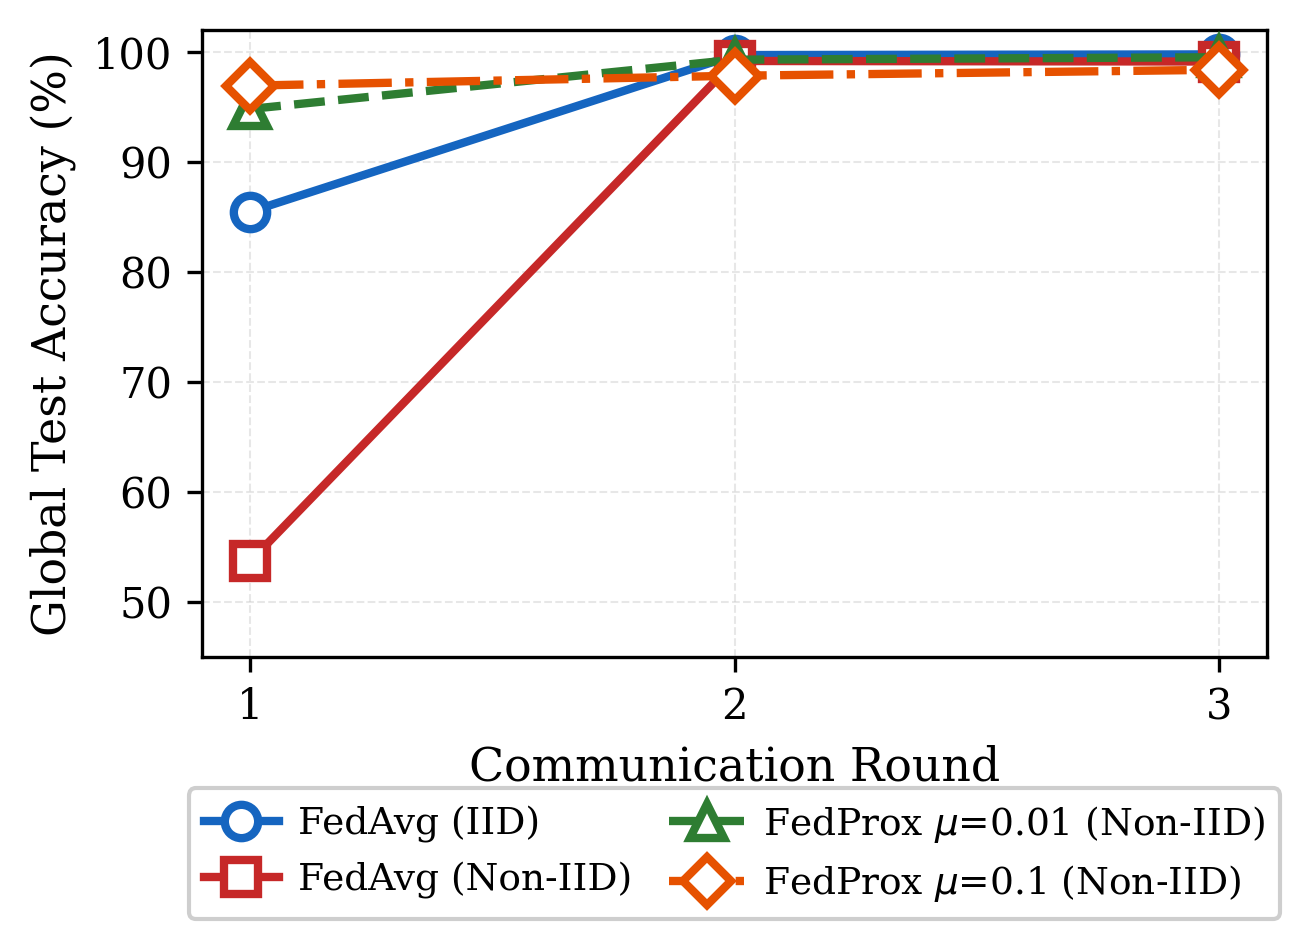
\includegraphics[width=\columnwidth]{figures/fig1_convergence_accuracy}
\caption{Global validation accuracy convergence for 3-node FL configurations under the image-level-split (v1) protocol. \todo{Regenerate with the group-level split, five seeds and shaded 95\% CI bands.}}
\label{fig:convergence}
\end{figure}

\begin{figure}[t]
\centering
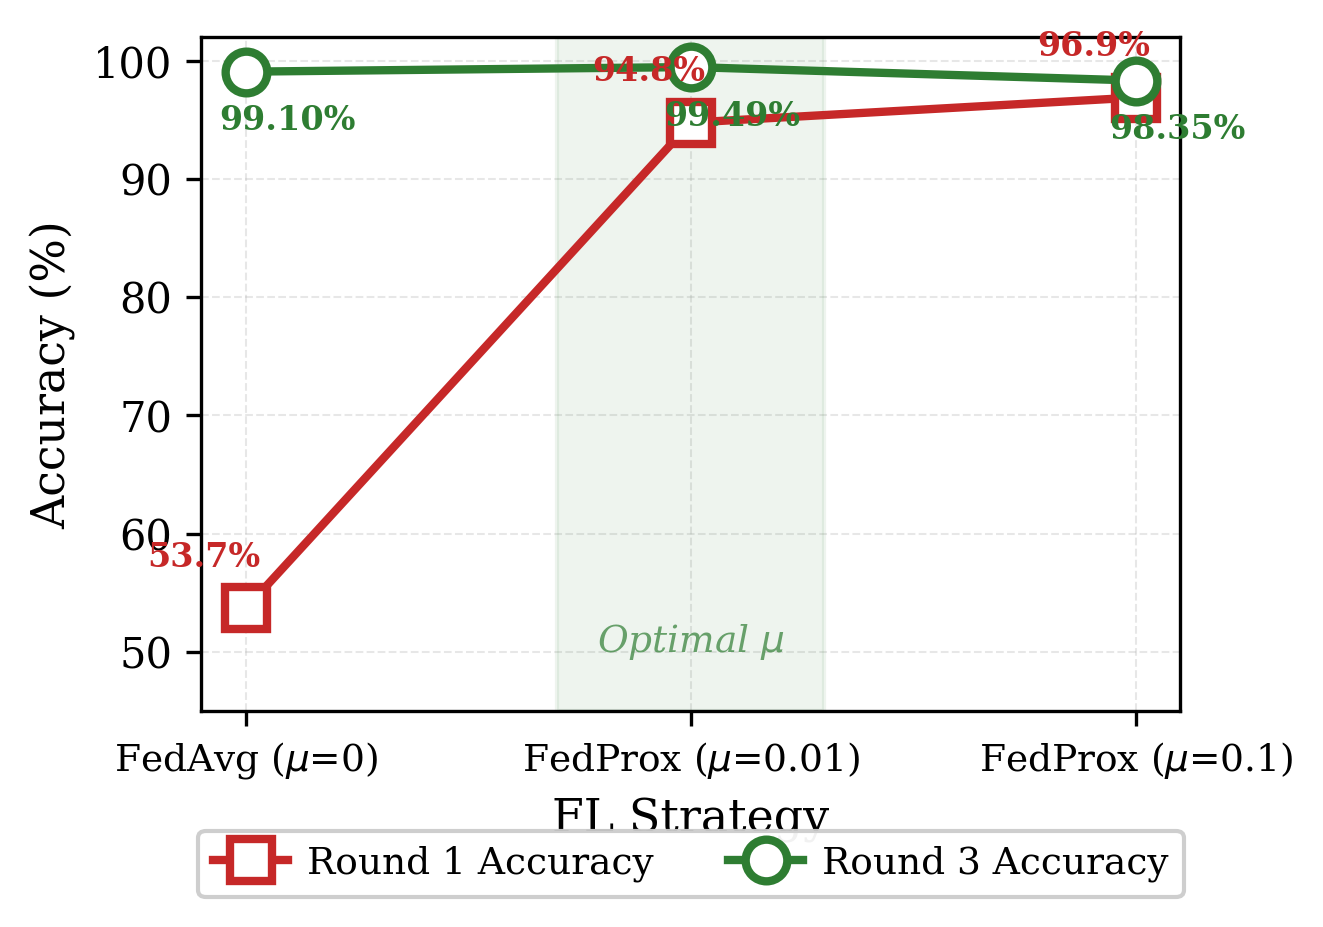
\includegraphics[width=\columnwidth]{figures/fig6_mu_tradeoff}
\caption{Proximal-term trade-off under the v1 protocol: increasing $\mu$ raises round-1 accuracy but lowers final accuracy. \todo{Extend to the full grid $\mu \in \{0.001, 0.01, 0.05, 0.1, 0.5\}$ (Section~\ref{sec:res_sensitivity}).}}
\label{fig:mu_tradeoff}
\end{figure}

\subsubsection{Per-Node Analysis Under Non-IID}

Table~\ref{tab:per_node} shows that the non-IID first-round degradation concentrates on the nodes with the strongest majority-class bias. Nodes~A (80\% fire) and B (88.5\% fire) reach only 45.11\% and 48.69\% round-1 accuracy with \fedavg{}, because their locally trained models fail on the minority class; Node~C (20\% fire), which observes the minority class more often, reaches 85.92\%.\todo{revisit: IID also collapses at round 1 under the group-level split} \fedprox{} ($\mu=0.01$) raises the weakest node from 45.11\% to 93.48\%. These are single-seed accuracies; the corresponding balanced accuracies, per-class sensitivities and confusion matrices under the revised protocol are reported in Section~\ref{sec:res_metrics}, and they are the quantities that actually identify \emph{which} class each node fails on.

\begin{table}[t]
\centering
\caption{Per-Node Accuracy (\%) Under Manual Non-IID Label Skew (3-Node, Image-Level Split, Seed 42)}
\label{tab:per_node}
\begin{tabular}{@{}llccc@{}}
\toprule
\textbf{Strategy} & \textbf{Round} & \textbf{Node A} & \textbf{Node B} & \textbf{Node C} \\
 & & \textbf{(80\% F)} & \textbf{(88.5\% F)} & \textbf{(20\% F)} \\
\midrule
\multirow{2}{*}{\fedavg{}} & R1 & 45.11 & 48.69 & 85.92 \\
 & R3 & 99.02 & 98.92 & 99.71 \\
\midrule
\multirow{2}{*}{\fedprox{} $\mu$=0.01} & R1 & 93.48 & 94.61 & 98.33 \\
 & R3 & 99.58 & 99.37 & 99.58 \\
\midrule
\multirow{2}{*}{\fedprox{} $\mu$=0.1} & R1 & 96.93 & 97.27 & 96.00 \\
 & R3 & 98.21 & 98.07 & 99.38 \\
\bottomrule
\end{tabular}
\end{table}

\begin{figure}[t]
\centering
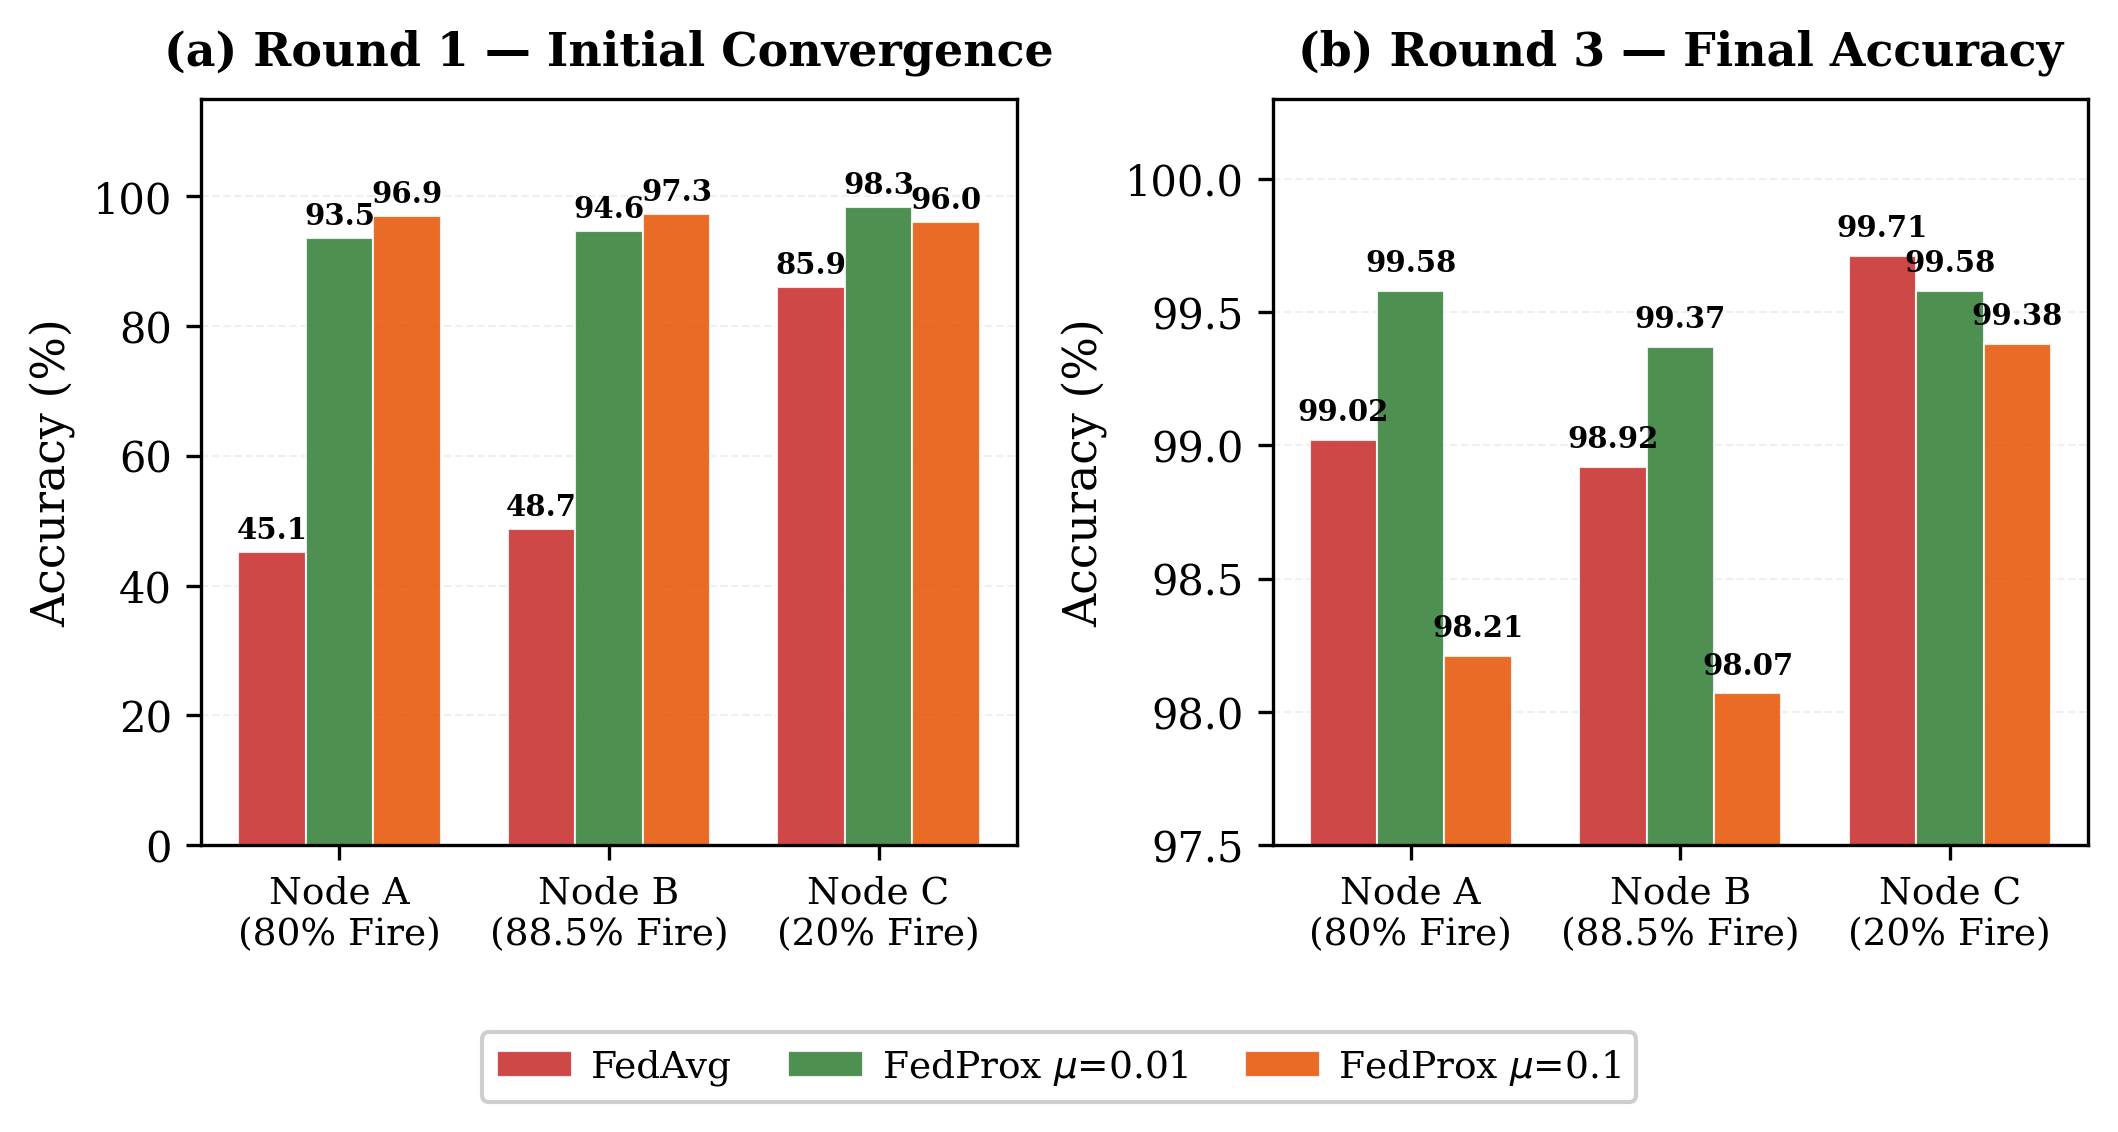
\includegraphics[width=\columnwidth]{figures/fig4_per_node_noniid}
\caption{Per-node accuracy under manual label skew (v1 protocol, seed~42). \todo{Regenerate as per-node balanced accuracy with CI bands under the group-level split.}}
\label{fig:pernode}
\end{figure}

\subsubsection{2-Node vs.\ 3-Node Scaling}

Fig.~\ref{fig:2v3} compares the 2-node and 3-node configurations of the v1 protocol. For the reference seed, adding a third node lowers round-1 accuracy by 13.34 points under IID (98.79\% $\to$ 85.45\%) and by 24.70 points under non-IID (78.36\% $\to$ 53.66\%), while the round-3 accuracies remain comparable. Given the seed variability quantified above, we present this as a consistent direction rather than as a calibrated effect size, and we do not extrapolate the trend to larger federations.

\begin{figure}[t]
\centering
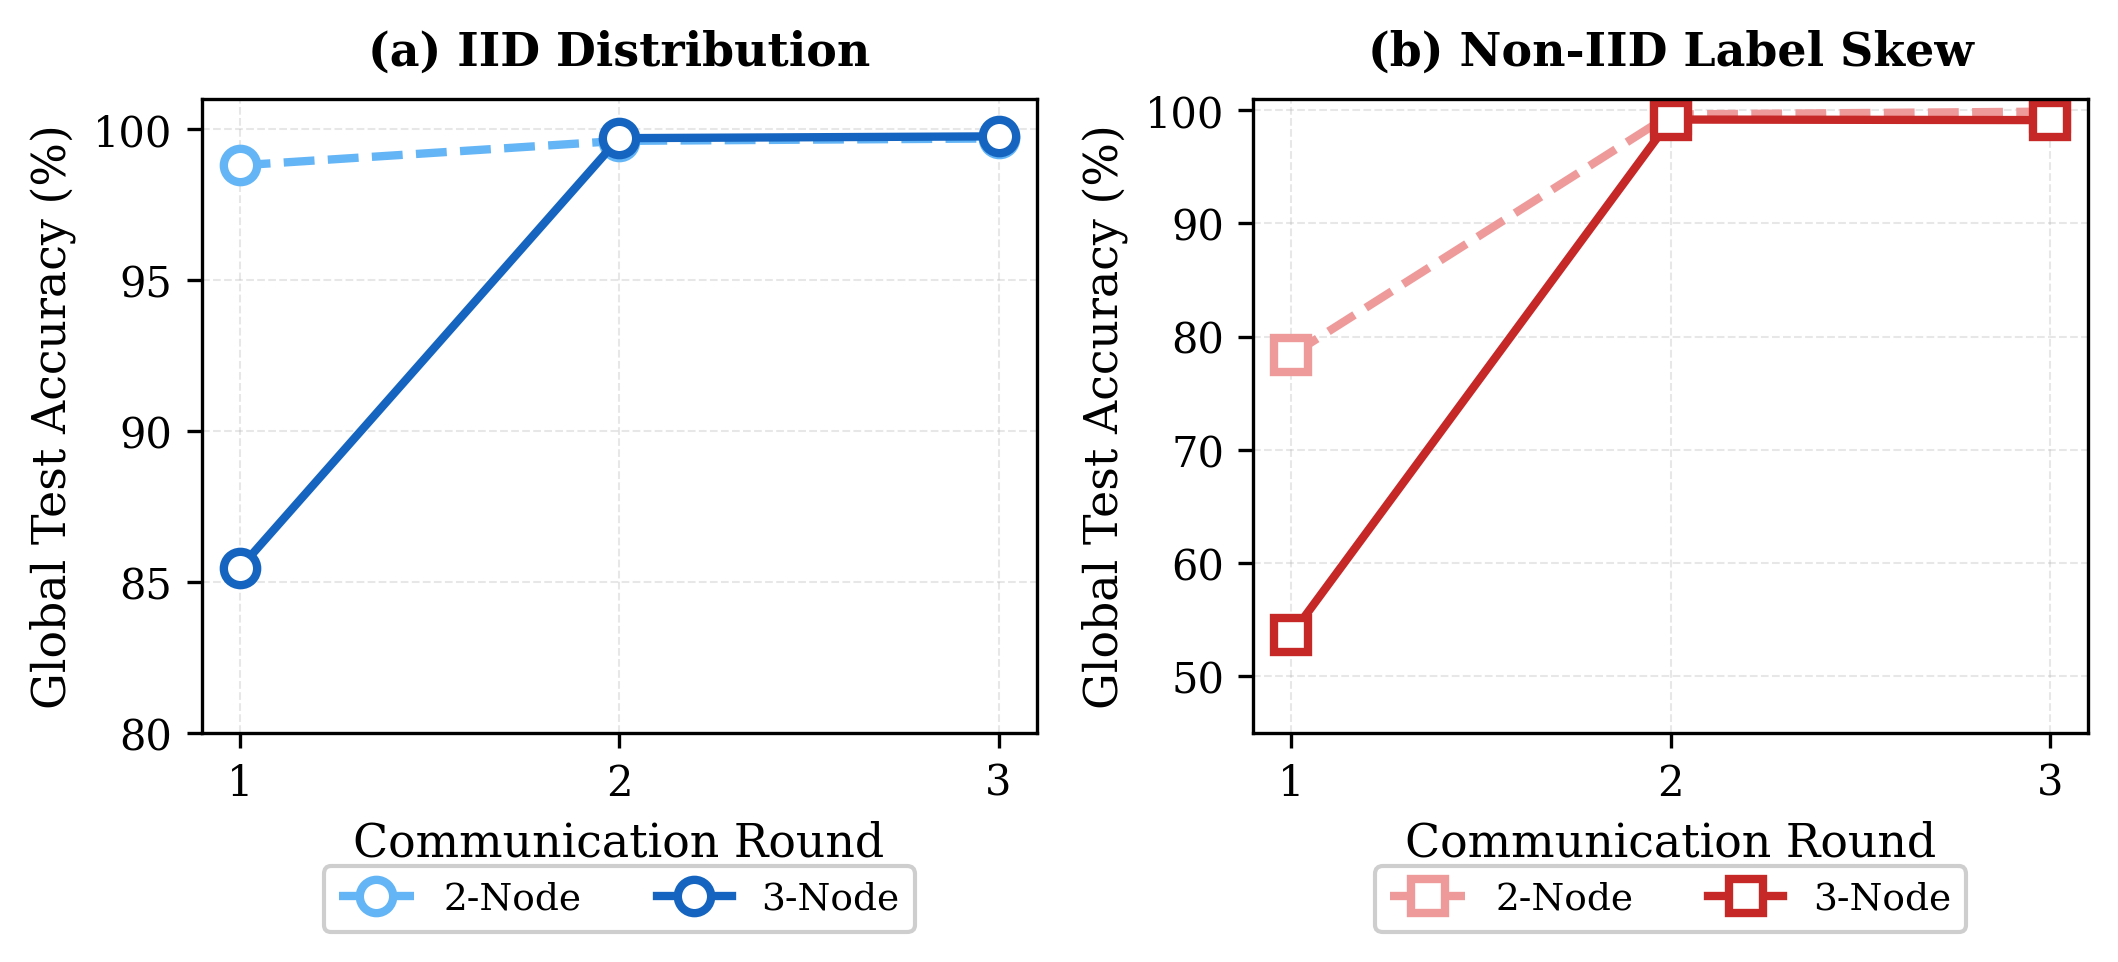
\includegraphics[width=\columnwidth]{figures/fig3_2node_vs_3node}
\caption{Effect of client count on first-round accuracy under (a)~IID and (b)~manual label skew, image-level-split protocol, reference seed. \todo{Add seed-aggregated bars with 95\% CIs.}}
\label{fig:2v3}
\end{figure}

\subsection{Leakage Audit and the Sequence-Level Split}
\label{sec:res_leakage}

Table~\ref{tab:leakage} reports the near-duplicate audit of the FLAME frames and of the two partitioning protocols. The result settles the reviewers' concern in the strongest possible way: under the v1 image-level split, 99.6\% of all validation and test images have a near-duplicate in the training split of some node, and 235 (IID) and 219 (label skew) of the 265 non-trivial groups were spread over several nodes. The near-perfect v1 accuracies of Section~\ref{sec:res_v1} therefore measure, to a large extent, recognition of sequences seen during training. Under the group-level protocol the independent audit of all 15 written partitions (IID, label skew, three Dirichlet skews, and their two low-data variants each) finds $L=0$ at $\tau=8$, the definition used to build the partitions, and no group spanning two nodes. Beyond the threshold the picture is continuous rather than clean (Table~\ref{tab:nn_distance}): some held-out images have a training image just above $\tau=8$ under dHash, and under pHash some fall within 8 bits. They are concentrated in a few pairs of adjacent segments of the same flight. Merging groups more aggressively does not remove this residual, and it is not free. Table~\ref{tab:grouping_tradeoff} rebuilds all five partitions under three coarser groupings, formed by unioning the dHash edges at $\tau=8$ with the pHash edges at 3, 4 and 6 bits. Adding pHash at 6 bits is the one that buys something: it cuts the dHash 9--10 residual from 188--476 images to 65--91. It pays for that by merging the 265 non-trivial groups down to 152, which costs on both of the other criteria---the smallest held-out set left to any client falls from 137 images to 116, and the number of per-node held-out class sets in which a single sequence supplies 90\% or more of the images rises from 2 of 55 to 8 of 53, so exactly the concentration that makes per-node metrics unreliable (Section~\ref{sec:limitations}) gets worse. The intermediate thresholds are not even reliably better on the residual they were meant to fix: at 4 bits the Dirichlet $\alpha{=}1$ partition improves only from 473 to 406 images, and at 3 bits it degrades to 520, because re-partitioning under a coarser grouping also reshuffles which images are held out at all. There is therefore no threshold that dominates the others, and we keep $\tau=8$ as the choice that is best on balance and on sequence dominance while leaving a residual that is measured rather than assumed, and handled by the clean-subset analysis of Section~\ref{sec:clean}. Table~\ref{tab:group_counts} lists the achieved per-node counts: the equal and label-skew designs are met to within a few dozen images, the Dirichlet skews are as extreme as intended (a node with 9\% fire next to a node with 95\%; one client with 911 images next to one with 41{,}786), and every client keeps at least 137 validation and 137 test images.

\begin{table}[t]
\centering
\caption{Near-Duplicate Audit of FLAME and of the Two Partitioning Protocols (dHash, $\tau=8$ bits, 47{,}992 images)}
\label{tab:leakage}
\setlength{\tabcolsep}{4pt}
\begin{tabular}{@{}lcc@{}}
\toprule
\multicolumn{3}{@{}l}{\textit{(a) Dataset}} \\
\midrule
Near-duplicate groups (non-trivial / all) & \multicolumn{2}{c}{265 / 394} \\
Images in non-trivial groups & \multicolumn{2}{c}{47{,}863 (99.73\%)} \\
Largest group (images) & \multicolumn{2}{c}{4{,}924} \\
Images sharing an identical hash & \multicolumn{2}{c}{31{,}979} \\
Byte-identical files & \multicolumn{2}{c}{39} \\
Cross-label groups (images) & \multicolumn{2}{c}{22 (20{,}006)} \\
Consecutive frame pairs in one group & \multicolumn{2}{c}{99.06\%} \\
\midrule
\multicolumn{3}{@{}l}{\textit{(b) Threshold sweep: groups / largest / images with a near-duplicate}} \\
\midrule
$\tau=4$ & \multicolumn{2}{c}{2{,}051 / 4{,}252 / 97.6\%} \\
$\tau=6$ & \multicolumn{2}{c}{927 / 4{,}255 / 99.1\%} \\
$\tau=8$ (used) & \multicolumn{2}{c}{394 / 4{,}924 / 99.7\%} \\
$\tau=10$ & \multicolumn{2}{c}{140 / 34{,}337 / 99.9\%} \\
$\tau=12$ & \multicolumn{2}{c}{41 / 46{,}294 / 100.0\%} \\
\midrule
\multicolumn{3}{@{}l}{\textit{(c) Partitioning protocol}} \\
 & \textbf{Image-level (v1)} & \textbf{Group-level} \\
\midrule
Leak rate $L$, Eq.~\eqref{eq:leak}, val / test (\%), IID & 99.64 / 99.65 & 0.00 / 0.00 \\
Leak rate $L$, val / test (\%), label skew & 99.58 / 99.65 & 0.00 / 0.00 \\
Leak rate $L$ (\%), Dirichlet and low-data partitions & -- & 0.00 \\
Groups spanning $>1$ node, IID / label skew & 235 / 219 & 0 / 0 \\
Worst per-node test leak rate (\%) & 99.88 & 0.00 \\
\bottomrule
\end{tabular}
\vspace{2pt}
\footnotesize{Parts (a) and (b) are properties of the dataset and the hash; part (c) audits the written partitions (\texttt{analysis/leakage/}). The leak rate $L$ is defined at $\tau=8$ (Eq.~\eqref{eq:leak}); the distances of held-out images beyond the threshold are given in Table~\ref{tab:nn_distance}. The v1 column is the image-level split of the original submission regenerated with its published seed; the group-level column covers all 15 partitions used in the revision. Groups are label-agnostic (Section~\ref{sec:leakage}).}
\end{table}

\IfFileExists{tables/nn_distance.tex}{\input{tables/nn_distance.tex}}{}

\IfFileExists{tables/grouping_tradeoff.tex}{% generated by scripts/grouping_tradeoff.py -- do not edit by hand
\begin{table}[t]
\centering
\caption{Effect of a Coarser Near-Duplicate Grouping on the Residual, the Balance and the Sequence Dominance of the Partitions. Ranges are over the Five Partitions (IID, Label Skew, Three Dirichlet Skews)}
\label{tab:grouping_tradeoff}
\small
\begin{tabular}{@{}lrrrrr@{}}
\toprule
\textbf{Grouping} & \textbf{Groups} & \textbf{Largest} & \textbf{dHash 9--10} & \textbf{Min held-out} & \textbf{Sets $\ge$90\%} \\
 & (non-triv.) & group & residual & per client & one sequence \\
\midrule
$\tau{=}8$ & 265 & 4924 & 188--476 & 137 & 2/55 \\
$\tau{=}8$ + pHash$\le$6 & 152 & 5103 & 65--91 & 116 & 8/53 \\
$\tau{=}8$ + pHash$\le$4 & 207 & 5030 & 127--408 & 137 & 7/53 \\
$\tau{=}8$ + pHash$\le$3 & 247 & 4924 & 125--520 & 137 & 5/56 \\
\bottomrule
\end{tabular}
\par\smallskip
\footnotesize A grouping is the connected components of the dHash edges at $\tau{=}8$, unioned with the pHash edges at the stated threshold; groups only ever merge. \textbf{dHash 9--10 residual}: held-out images whose nearest training image (any node) falls in that band, summed over validation and test, range over the five partitions. \textbf{Min held-out per client}: the smallest validation or test set any client is left with. \textbf{Sets $\ge$90\% one sequence}: per-node held-out class sets of at least 50 images in which a single sequence supplies 90\% or more of the images, out of all such sets in the five partitions. Every row is rebuilt by the same code path, and the $\tau{=}8$ row reproduces the shipped partition exactly (\texttt{scripts/grouping\_tradeoff.py --check-shipped}).
\end{table}
}{}

\IfFileExists{tables/heldout_sequences.tex}{% generated by scripts/heldout_dominance.py -- do not edit by hand
\begin{table}[t]
\centering
\caption{Held-Out Sequences per Class (Validation / Test), by Partition and Node. A Class Carried by One or Two Sequences Has No Between-Sequence Variance for the Bootstrap to Estimate}
\label{tab:heldout_sequences}
\small
\begin{tabular}{@{}llrrrr@{}}
\toprule
\textbf{Partition} & \textbf{Node} & \multicolumn{2}{c}{\textbf{Fire}} & \multicolumn{2}{c}{\textbf{No-fire}} \\
\cmidrule(lr){3-4} \cmidrule(lr){5-6}
 & & val & test & val & test \\
\midrule
IID & node\_a & 23 & 21 & 33 & \textbf{2}$^{\dagger}$ \\
 & node\_b & 21 & 10 & 34 & 34 \\
 & node\_c & 21 & 22 & 23 & 24 \\
\addlinespace
Label skew & node\_a & 22 & 22 & 23 & 22 \\
 & node\_b & 33 & 31 & 22 & 22 \\
 & node\_c & 18 & 23 & 25 & 26 \\
\addlinespace
Dir.\ $\alpha{=}0.1$ & node\_a & 3 & 3 & 69 & 68 \\
 & node\_b & 29 & 31 & \textbf{2}$^{\dagger}$ & \textbf{2}$^{\dagger}$ \\
 & node\_c & 29 & 30 & \textbf{1}$^{\dagger}$ & \textbf{1}$^{\dagger}$ \\
\addlinespace
Dir.\ $\alpha{=}0.5$ & node\_a & 26 & 26 & 16 & 16 \\
 & node\_b & 24 & 25 & 41 & 43 \\
 & node\_c & 18 & 19 & 3 & 3 \\
\addlinespace
Dir.\ $\alpha{=}1$ & node\_a & 21 & 20 & 25 & 25 \\
 & node\_b & 21 & 21 & 22 & 21 \\
 & node\_c & 20 & 22 & 23 & 21 \\
\addlinespace
\bottomrule
\end{tabular}
\par\smallskip
\footnotesize Number of distinct near-duplicate groups (sequences) contributing to each held-out class set. $^{\dagger}$ marks a class carried by at most 2 sequences: the sequence-level bootstrap can then no longer estimate between-sequence variance for that class, so the interval is conditional on those particular videos and understates uncertainty about new footage. The count matters independently of the number of images -- in the IID partition node~A's 1{,}011 no-fire test images are two sequences. The low-data variants subsample only the training split and have the same held-out cells. Produced by \texttt{scripts/heldout\_dominance.py}.
\end{table}
}{}

\begin{table}[t]
\centering
\caption{Achieved Per-Node Counts of the Group-Level Partitions (3 Nodes, Seed 42): Train / Val / Test Images and Fire Share}
\label{tab:group_counts}
\setlength{\tabcolsep}{3pt}
\begin{tabular}{@{}llrrrr@{}}
\toprule
\textbf{Partition} & \textbf{Node} & \textbf{Train} & \textbf{Val} & \textbf{Test} & \textbf{Fire (\%)} \\
\midrule
\multirow{3}{*}{IID} & A & 11{,}139 & 2{,}340 & 2{,}519 & 62.8 \\
 & B & 11{,}346 & 2{,}326 & 2{,}326 & 62.8 \\
 & C & 11{,}196 & 2{,}400 & 2{,}400 & 62.8 \\
\midrule
\multirow{3}{*}{Label skew} & A & 11{,}197 & 2{,}400 & 2{,}400 & 80.0 \\
 & B & 11{,}201 & 2{,}399 & 2{,}398 & 88.5 \\
 & C & 11{,}197 & 2{,}400 & 2{,}400 & 20.0 \\
\midrule
\multirow{3}{*}{Dirichlet $\alpha=0.1$} & A & 11{,}971 & 2{,}586 & 2{,}647 & 9.0 \\
 & B & 14{,}199 & 3{,}178 & 2{,}959 & 95.2 \\
 & C & 7{,}462 & 1{,}392 & 1{,}598 & 88.4 \\
\midrule
\multirow{3}{*}{Dirichlet $\alpha=0.5$} & A & 3{,}706 & 794 & 795 & 97.0 \\
 & B & 29{,}249 & 6{,}268 & 6{,}269 & 57.7 \\
 & C & 637 & 137 & 137 & 97.8 \\
\midrule
\multirow{3}{*}{Dirichlet $\alpha=1.0$} & A & 11{,}168 & 2{,}393 & 2{,}394 & 18.5 \\
 & B & 14{,}939 & 3{,}201 & 3{,}202 & 88.7 \\
 & C & 7{,}486 & 1{,}604 & 1{,}605 & 77.4 \\
\bottomrule
\end{tabular}
\vspace{2pt}
\footnotesize{Low-data variants keep the validation and test columns and reduce the training column to $\rho$ of its size at frame level: $557$--$568$ images per node at $\rho=0.05$ and $111$--$113$ at $\rho=0.01$ for the IID and label-skew partitions. Targets: 11{,}198 / 2{,}400 / 2{,}400 per node for IID and label skew; the deviations are the cost of assigning whole sequences. Full per-class tables: \texttt{data/processed/split\_stats.json}.}
\end{table}

\begin{table}[t]
\centering
\caption{Effect of the Partitioning Protocol on the Reported \emph{Accuracy} (3-Node, mean $\pm$ std over seeds). Accuracy is the secondary metric of this study (Section~\ref{sec:primary}); it is the quantity shown here because the comparison is precisely about how much accuracy the leaked protocol added. Balanced accuracy, the primary metric, is in Table~\ref{tab:fullmetrics}}
\label{tab:protocol_effect}
\begin{tabular}{@{}llcc@{}}
\toprule
\textbf{Dist.} & \textbf{Method} & \textbf{Image-level (\%)} & \textbf{Group-level (\%)} \\
\midrule
\multirow{5}{*}{IID}
 & Centralized     & $99.65 \pm 0.13$ ($n{=}3$) & $93.4 \pm 1.2$ ($n{=}5$) \\
 & Local-only      & $99.49 \pm 0.08$ ($n{=}3$) & $86.9 \pm 1.4$ ($n{=}5$) \\
 & \fedavg{}       & $99.32 \pm 0.03$ ($n{=}2$) & $\PH \pm \PH$ \\
 & \fedprox{} 0.01 & $99.18 \pm 0.12$ ($n{=}3$) & $\PH \pm \PH$ \\
 & \fedbn{}        & $95.69 \pm 3.12$ ($n{=}3$) & $\PH \pm \PH$ \\
\midrule
\multirow{5}{*}{Non-IID}
 & Centralized     & $99.72 \pm 0.07$ ($n{=}3$) & $94.3 \pm 1.6$ ($n{=}5$) \\
 & Local-only      & $99.50 \pm 0.03$ ($n{=}3$) & $95.5 \pm 0.8$ ($n{=}5$) \\
 & \fedavg{}       & $99.31 \pm 0.39$ ($n{=}3$) & $\PH \pm \PH$ \\
 & \fedprox{} 0.01 & $99.22 \pm 0.24$ ($n{=}3$) & $\PH \pm \PH$ \\
 & \fedbn{}        & $75.06 \pm 8.36$ ($n{=}3$) & $\PH \pm \PH$ \\
\bottomrule
\end{tabular}
\vspace{2pt}
\footnotesize{The two columns are \emph{not} paired: they use different partitions and different seed sets. Image-level values are the v1 results of Table~\ref{tab:v1_ci} (validation accuracy for the federated rows, test accuracy for the baselines); every group-level cell, baseline and federated alike, is test accuracy at the round (baselines: epoch) selected by the rule of Section~\ref{sec:selection}. Local-only Non-IID accuracy is inflated by the class imbalance of each node's own test split; balanced accuracy is $88.6 \pm 1.8$ against $94.7 \pm 0.9$ for the centralized model (Table~\ref{tab:fullmetrics}). All group-level numbers are produced by \texttt{scripts/analyze\_results.py} into \texttt{analysis/summary\_table.csv} and are pinned to it by \texttt{tests/test\_paper\_numbers.py}. \todo{Fill the federated group-level cells from the \texttt{rev\_*} Jetson runs.}}
\end{table}

\subsection{Full Metric Set and Per-Client Confusion Matrices}
\label{sec:res_metrics}

The two reference conditions have been run under the audited protocol (Table~\ref{tab:fullmetrics}; five seeds, desktop GPU, Jetson hyperparameters). Removing the sequence leakage moves the centralized reference from 99.7\% to $93.4 \pm 1.2$\% (IID) and $94.3 \pm 1.6$\% (label skew) test accuracy, and the local-only reference from 99.5\% to $86.9 \pm 1.4$\% and $95.5 \pm 0.8$\%. Two consequences follow for the rest of the paper. First, the task is no longer saturated: the gap between the two references is 6.5 points of accuracy under IID and 6.1 points of balanced accuracy under label skew, which is the room in which a federated strategy can show whether it helps.\todo{Revisit after the FL results: the size of this band, and every claim below that depends on it, must be written against where the federated strategies actually land inside it.} Second, the accuracy-only view that the reviewers criticised is misleading exactly where it matters. Under label skew the local-only models reach a \emph{higher} accuracy than the centralized model ($95.5$\% vs.\ $94.3$\%) while their balanced accuracy, specificity and MCC are clearly lower ($88.6$ vs.\ $94.7$, $83.8$ vs.\ $96.4$, $0.81$ vs.\ $0.88$), because a node that trains on 80--88\% fire frames rarely predicts no-fire and is tested on an equally skewed split; accuracy alone would rank the wrong method first.\todo{Revisit after the FL results: this is now an accuracy inversion, not a tie, and the sentence should be written against the federated rows once they exist.} Table~\ref{tab:protocol_effect} places the two protocols side by side.

The reporting protocol itself accounts for a large part of the reference gap, which is a finding about how such results are reported rather than a result about federation. Selecting the epoch by validation loss instead of reporting the final epoch raises the IID centralized reference from $90.9 \pm 2.4$\% to $93.4 \pm 1.2$\% and the local-only reference from $78.3 \pm 5.0$\% to $86.9 \pm 1.4$\%, so the centralized-to-local-only gap narrows from 12.6 to 6.5 points: final-epoch reporting more than doubles the apparent advantage of pooling the data. The effect is asymmetric because the local-only models are the unstable ones across epochs---on node~C the validation accuracy of the local-only IID baseline moves between 0.96 and 0.42 in consecutive epochs while its training loss stays below 0.05 (\texttt{results/rev\_baselines\_sel/rev\_iid\_local\_seed123})---so a final-epoch snapshot penalises them far more often than it penalises the pooled model. Both protocols are kept in the repository under separate labels (\texttt{group} and \texttt{group\_final\_epoch} in \texttt{analysis/runs.csv}); everything reported in this paper uses the declared selection rule.

\begin{table*}[t]
\centering
\caption{Test-Set Metrics Under the Group-Level Split (3-Node, mean $\pm$ std, $n=5$ Seeds; Percentages Except MCC)}
\label{tab:fullmetrics}
\begin{tabular}{@{}llccccccc@{}}
\toprule
\textbf{Dist.} & \textbf{Method} & \textbf{Bal.\ acc.} & \textbf{MCC} & \textbf{Acc.} & \textbf{Sens.} & \textbf{Spec.} & \textbf{Macro-}$F_1$ & \textbf{ROC-AUC} \\
\midrule
\multirow{5}{*}{IID}
 & Centralized      & $93.7 \pm 1.4$ & $0.86 \pm 0.03$ & $93.4 \pm 1.2$ & $92.3 \pm 1.3$ & $95.2 \pm 2.4$ & $93.1 \pm 1.3$ & $98.0 \pm 0.3$ \\
 & Local-only$^{\dagger}$ & $84.5 \pm 1.5$ & $0.73 \pm 0.02$ & $86.9 \pm 1.4$ & $91.9 \pm 3.8$ & $77.1 \pm 5.2$ & $85.0 \pm 1.6$ & $94.2 \pm 1.2$ \\
 & \fedavg{}        & \PHs & \PHs & \PHs & \PHs & \PHs & \PHs & \PHs \\
 & \fedprox{} 0.01  & \PHs & \PHs & \PHs & \PHs & \PHs & \PHs & \PHs \\
 & \fedbn{}         & \PHs & \PHs & \PHs & \PHs & \PHs & \PHs & \PHs \\
\midrule
\multirow{5}{*}{Non-IID}
 & Centralized      & $94.7 \pm 0.9$ & $0.88 \pm 0.03$ & $94.3 \pm 1.6$ & $93.0 \pm 3.7$ & $96.4 \pm 2.0$ & $94.0 \pm 1.6$ & $99.3 \pm 0.2$ \\
 & Local-only       & $88.6 \pm 1.8$ & $0.81 \pm 0.03$ & $95.5 \pm 0.8$ & $93.5 \pm 2.2$ & $83.8 \pm 2.6$ & $90.1 \pm 1.6$ & $95.1 \pm 1.7$ \\
 & \fedavg{}        & \PHs & \PHs & \PHs & \PHs & \PHs & \PHs & \PHs \\
 & \fedprox{} 0.01  & \PHs & \PHs & \PHs & \PHs & \PHs & \PHs & \PHs \\
 & \fedbn{}         & \PHs & \PHs & \PHs & \PHs & \PHs & \PHs & \PHs \\
\bottomrule
\end{tabular}
\vspace{2pt}
\parbox{\textwidth}{\footnotesize Every row is the test metric at the round (baselines: epoch) selected by the rule of Section~\ref{sec:selection}; the selection uses the aggregated validation loss only. Centralized: pooled training data, pooled test split. Local-only: each node trained and tested on its own split, metrics averaged over the three nodes (metrics defined in Eqs.~\eqref{eq:acc}--\eqref{eq:auc}). Under label skew the local-only \emph{accuracy} matches the centralized model while its specificity and MCC fall, because a node that sees 80--88\% fire rarely predicts no-fire and is evaluated on an equally skewed test split; balanced accuracy and MCC are the metrics that expose this. Both baselines were trained on a desktop GPU with the Jetson hyperparameters (batch~8, Adam $10^{-3}$, 15 epochs), so their timing is not comparable to the federated rows. $^{\dagger}$ marks a row in which some evaluated client's minority class is carried by at most two held-out sequences (Table~\ref{tab:heldout_sequences}): under IID, node~A's 1{,}011 no-fire test images are two sequences, so the per-client uncertainty of that row is conditional on those two videos (Section~\ref{sec:limitations}). The centralized rows pool the three nodes' held-out splits and are not affected. \todo{Fill the federated rows from the \texttt{rev\_*} Jetson runs (\texttt{analysis/summary\_table.md}) and add the 95\% CIs.}}
\end{table*}

\begin{table}[t]
\centering
\caption{Per-Client Test Metrics at the Selected Round Under Manual Label Skew (Group-Level Split, $n=5$)}
\label{tab:perclient_metrics}
\setlength{\tabcolsep}{4pt}
\begin{tabular}{@{}llcccc@{}}
\toprule
\textbf{Method} & \textbf{Node} & \textbf{Bal.\ acc.} & \textbf{Sens.} & \textbf{Spec.} & \textbf{MCC} \\
\midrule
\multirow{3}{*}{\fedavg{}}
 & A (80\% F)   & \PHs & \PHs & \PHs & \PHs \\
 & B (88.5\% F) & \PHs & \PHs & \PHs & \PHs \\
 & C (20\% F)   & \PHs & \PHs & \PHs & \PHs \\
\midrule
\multirow{3}{*}{\fedprox{} 0.01}
 & A & \PHs & \PHs & \PHs & \PHs \\
 & B & \PHs & \PHs & \PHs & \PHs \\
 & C & \PHs & \PHs & \PHs & \PHs \\
\midrule
\multirow{3}{*}{\fedbn{}}
 & A & \PHs & \PHs & \PHs & \PHs \\
 & B & \PHs & \PHs & \PHs & \PHs \\
 & C & \PHs & \PHs & \PHs & \PHs \\
\bottomrule
\end{tabular}
\vspace{2pt}
\footnotesize{\todo{Fill from the per-client rows of \texttt{results.json}; add rounds 1 and 3 on the \emph{validation} split so that the recovery of the minority-class sensitivity over rounds is visible; test metrics are reported only at the selected round (Section~\ref{sec:selection}).}}
\end{table}

\begin{figure}[t]
\centering
\todo{Figure: per-client confusion matrices (3 nodes $\times$ \{round 1 on validation, selected round on test\}) for \fedavg{}, \fedprox{}~0.01 and \fedbn{} under manual label skew, normalised by true class. Produced by \texttt{scripts/analyze\_results.py}.}
\caption{Per-client confusion matrices under manual label skew, showing which class each client fails on in the first round and to what extent aggregation repairs it.}
\label{fig:confmat}
\end{figure}

\subsection{Dirichlet Label Skew}
\label{sec:res_dirichlet}

Table~\ref{tab:dirichlet} reports the reference conditions on the three Dirichlet partitions of Table~\ref{tab:group_counts}. The local-only reference degrades with the skew as intended: at $\alpha=0.1$, where two nodes hold fire frames only, the node-averaged balanced accuracy is $58.7$\% (accuracy $90.7$\%, i.e.\ a majority-class predictor on a skewed test split), at $\alpha=0.5$ it is $80.1$\% and at $\alpha=1.0$ $87.7$\%. The centralized model is trained on the same pooled frames in all three columns, so its variation between $90.5$\% and $76.0$\% is caused by which sequences each partition holds out for testing rather than by the skew; we return to this in Section~\ref{sec:limitations}. The federated rows will show whether aggregation recovers the minority class that the $\alpha=0.1$ clients never see locally.

\begin{table}[t]
\centering
\caption{Test Balanced Accuracy (\%) at the Selected Round Under Dirichlet Label Skew (3-Node, Group-Level Split, mean [95\% CI], $n=3$ Seeds)}
\label{tab:dirichlet}
\begin{tabular}{@{}lccc@{}}
\toprule
\textbf{Method} & $\alpha=0.1$ & $\alpha=0.5$ & $\alpha=1.0$ \\
\midrule
Centralized     & 90.5 [81.0, 99.9] & 88.8 [72.4, 100] & 76.0 [71.1, 80.9] \\
Local-only      & 58.7 [50.0, 67.4] & 80.1 [60.3, 100] & 87.7 [76.4, 99.0] \\
\fedavg{}       & \PHs & \PHs & \PHs \\
\fedprox{} 0.01 & \PHs & \PHs & \PHs \\
\fedbn{}        & \PHs & \PHs & \PHs \\
\bottomrule
\end{tabular}
\vspace{2pt}
\footnotesize{Local-only values are averaged over the three nodes, each tested on its own split; the achieved per-node class counts are those of Table~\ref{tab:group_counts}. At $\alpha=0.1$ two nodes hold fire frames only and one holds 9\% fire, so a locally trained model predicts a single class on most of its test split (balanced accuracy near 50\%). The centralized model uses the same pooled training frames in every column; its spread (90.5 to 76.0) reflects which sequences the three partitions hold out for testing, not the skew. \todo{Fill the federated rows from the \texttt{dirichlet\_skew} block and state whether the ranking of the methods is preserved across $\alpha$.}}
\end{table}

\begin{figure}[t]
\centering
\todo{Figure: final balanced accuracy vs.\ Dirichlet concentration $\alpha$ (log axis), one line per strategy, with 95\% CI bands; a horizontal line marks the IID reference.}
\caption{Stability of the strategy ranking across the degree of label skew.}
\label{fig:dirichlet}
\end{figure}

\subsection{Low-Data Regime}
\label{sec:res_lowdata}

Table~\ref{tab:lowdata} reports the reference conditions at $\rho \in \{1, 0.05, 0.01\}$. Because the subsample is drawn at frame level inside each node's sequences (Section~\ref{sec:lowdata}), reducing a node from about 11{,}200 to 112 training frames costs the local-only model surprisingly little under IID (balanced accuracy $76.6$ to $80.4$\%, within the confidence intervals) and about eight points under label skew ($87.9$ to $79.8$\%); the centralized model loses two to four points. The near-duplicate structure of FLAME is the reason: a node's 112 frames still cover most of its sequences, so the regime removes redundant frames before it removes information. This is the conservative reading announced in Section~\ref{sec:lowdata}, and it means that a federated advantage in this table has to come from combining \emph{sequences} across nodes rather than from sample count alone.

\begin{table}[t]
\centering
\caption{Test Balanced Accuracy (\%) at the Selected Round in the Low-Data Regime (3-Node, Group-Level Split, mean [95\% CI])}
\label{tab:lowdata}
\setlength{\tabcolsep}{3pt}
\begin{tabular}{@{}llccc@{}}
\toprule
\textbf{Dist.} & \textbf{Method} & $\rho{=}1.00$ & $\rho{=}0.05$ & $\rho{=}0.01$ \\
\midrule
\multirow{4}{*}{IID}
 & Centralized     & 92.0 [89.5, 94.4] & 89.7 [79.0, 100] & 89.1 [82.7, 95.6] \\
 & Local-only      & 76.6 [71.6, 81.5] & 81.0 [78.0, 84.0] & 80.4 [79.1, 81.6] \\
 & \fedavg{}       & \PHs & \PHs & \PHs \\
 & \fedprox{} 0.01 & \PHs & \PHs & \PHs \\
\midrule
\multirow{4}{*}{Non-IID}
 & Centralized     & 94.5 [92.4, 96.6] & 91.6 [80.7, 100] & 90.8 [81.1, 100] \\
 & Local-only      & 87.9 [85.0, 90.8] & 85.3 [75.8, 94.8] & 79.8 [59.5, 100] \\
 & \fedavg{}       & \PHs & \PHs & \PHs \\
 & \fedprox{} 0.01 & \PHs & \PHs & \PHs \\
\bottomrule
\end{tabular}
\vspace{2pt}
\footnotesize{$\rho$ is the retained fraction of each node's training split, Eq.~\eqref{eq:subsample}; $n=5$ seeds at $\rho=1$, $n=3$ at $\rho=0.05$ and $0.01$. Training images per node: 11{,}139--11{,}346 ($\rho=1$), 557--568 ($\rho=0.05$), 111--113 ($\rho=0.01$). The centralized model pools the three reduced training splits (about 1{,}700 and 340 frames). \todo{Fill the federated rows from the \texttt{low\_data} block; the key quantity is the federated-minus-local gap as a function of $\rho$.}}
\end{table}

\subsection{Hyperparameter Sensitivity}
\label{sec:res_sensitivity}

\begin{table}[t]
\centering
\caption{Sensitivity of the Selected-Round Test Balanced Accuracy to the Local and Federation Hyperparameters (3-Node, Non-IID, mean [95\% CI])}
\label{tab:sensitivity}
\begin{tabular}{@{}llc@{}}
\toprule
\textbf{Factor} & \textbf{Setting} & \textbf{Final bal.\ acc.} \\
\midrule
\multirow{5}{*}{Proximal strength $\mu$}
 & 0.001 & \PHs \\
 & 0.01  & \PHs \\
 & 0.05  & \PHs \\
 & 0.1   & \PHs \\
 & 0.5   & \PHs \\
\midrule
\multirow{3}{*}{Local epochs $E$}
 & 1 & \PHs \\
 & 2 & \PHs \\
 & 5 & \PHs \\
\midrule
\multirow{2}{*}{Learning rate $\eta$}
 & $10^{-4}$ & \PHs \\
 & $10^{-3}$ & \PHs \\
\bottomrule
\end{tabular}
\vspace{2pt}
\footnotesize{One factor varied at a time about the default point ($\mu{=}0.01$, $E{=}5$, $\eta{=}10^{-3}$, batch~8). \todo{Fill from the \texttt{mu\_grid}, \texttt{local\_epochs} and \texttt{learning\_rate} blocks; add the matching round-1 column, because $\mu$ and $E$ affect the early rounds far more than the final round.}}
\end{table}

\begin{figure}[t]
\centering
\todo{Figure: three panels, final and round-1 balanced accuracy vs.\ (a)~$\mu$ (log axis), (b)~$E$, (c)~$\eta$, with 95\% CI bands.}
\caption{Hyperparameter sensitivity of the federated strategies under label skew.}
\label{fig:sensitivity}
\end{figure}

\subsection{Extended Communication Budget for FedBN}
\label{sec:res_fedbn}

Under the v1 three-round budget, \fedbn{} was the weakest method in both distributions and was markedly unstable under label skew ($75.06\% \pm 8.36\%$, 95\% CI $[54.30, 95.83]$, $n=3$). We deliberately do \emph{not} conclude from this that \fedbn{} is unsuitable for this task, nor that it would necessarily become competitive given more rounds: both statements exceed the evidence of a three-round experiment. The ten-round block of Table~\ref{tab:fedbn10} tests the second statement directly against a matched \fedavg{} reference.

\begin{table}[t]
\centering
\caption{\fedbn{} Under an Extended Communication Budget (3-Node, Group-Level Split, mean [95\% CI])}
\label{tab:fedbn10}
\begin{tabular}{@{}llcc@{}}
\toprule
\textbf{Dist.} & \textbf{Method} & \textbf{3-round run} & \textbf{10-round run} \\
\midrule
\multirow{2}{*}{IID}
 & \fedavg{} & \PHs & \PHs \\
 & \fedbn{}  & \PHs & \PHs \\
\midrule
\multirow{2}{*}{Non-IID}
 & \fedavg{} & \PHs & \PHs \\
 & \fedbn{}  & \PHs & \PHs \\
\bottomrule
\end{tabular}
\vspace{2pt}
\footnotesize{Test balanced accuracy at the round selected by the rule of Section~\ref{sec:selection} within each run's budget ($r^{*} \le 3$ and $r^{*} \le 10$). \todo{Fill from the \texttt{long\_horizon\_fedbn} block. State explicitly whether the \fedbn{}--\fedavg{} difference at R10 has a CI that excludes zero; if it does not, the conclusion is that ten rounds are still insufficient to separate them, not that they are equivalent.}}
\end{table}

\subsection{Time- and Communication-Normalised Comparison}
\label{sec:res_time}

Table~\ref{tab:time} reports the measured wall-clock cost and communication volume of the revision runs (group-level split, wired Gigabit Ethernet). \todo{From the \texttt{rev\_*} runs, state the three-round 3-node time of \fedavg{} and of \fedprox{} ($\mu=0.01$) under label skew and their ratio, with 95\% CIs. Do not reuse the v1 ratio.} Communication volume is identical for \fedavg{} and \fedprox{} ($110.3$\,MB cumulative over three rounds with $K=3$ and $|w| \approx 6.13$\,MB, in agreement with~\eqref{eq:comm}), because \fedprox{} changes the local objective and not the payload. The v1 runs of the original submission were timed over WiFi and under the image-level split; because both the network and the data partition have changed, v1 and revision wall-clock numbers are not comparable, and the v1 timings are superseded by, not extended with, the revision timings. They are therefore not reported here.

The distinction between cost per round and cost per second matters for the interpretation of the first-round advantage of \fedprox{}: an improvement that is obtained per \emph{round} is not necessarily an improvement per \emph{second}, so a fair claim requires the time-normalised curve of Fig.~\ref{fig:timecomm} rather than Table~\ref{tab:main_results}. \todo{From the \texttt{rev\_*} runs, state how the time \fedprox{} needs for its first round compares with the time \fedavg{} needs per round.}

\IfFileExists{tables/time.tex}{\input{tables/time.tex}}{%
\begin{table}[t]
\centering
\caption{Measured Total Training Time, Group-Level Split, Wired Gigabit Ethernet (3 Rounds)}
\label{tab:time}
\setlength{\tabcolsep}{2.5pt}
\begin{tabular}{@{}lccc@{}}
\toprule
\textbf{Configuration} & \textbf{Time (min)} & \textbf{Comm.\ (MB)} & \textbf{Test acc.\ (\%)} \\
\midrule
2N IID \fedavg{} & \PH & \PH & \PH \\
2N Non-IID \fedavg{} & \PH & \PH & \PH \\
3N IID \fedavg{} & \PH & \PH & \PH \\
3N Non-IID \fedavg{} & \PH & \PH & \PH \\
3N Non-IID \fedprox{} $\mu$=0.01 & \PH & \PH & \PH \\
3N Non-IID \fedbn{} & \PH & \PH & \PH \\
\bottomrule
\end{tabular}
\vspace{2pt}
\footnotesize{\todo{Placeholder. This table is generated by \texttt{scripts/export\_latex\_tables.py} as \texttt{paper/tables/time.tex} from the \texttt{rev\_*} runs and replaces this placeholder automatically once that file exists. v1 (WiFi, image-level split) timings are not included.}}
\end{table}}

\begin{figure}[t]
\centering
\IfFileExists{figures/fig_timecomm.pdf}{\includegraphics[width=\columnwidth]{figures/fig_timecomm}}{\fbox{\parbox[c][3cm][c]{0.9\columnwidth}{\centering\todo{three-panel figure}}}}
\caption{Accuracy versus communication round, elapsed wall-clock time and cumulative transmitted megabytes for the revision runs (group-level split, wired Gigabit Ethernet). v1 runs are not drawn: they were timed over WiFi and under a different partition, so their time axis is not comparable. \todo{Generate from the \texttt{rev\_*} runs with \texttt{scripts/analyze\_results.py}, which excludes image-level-split runs from the time and communication panels.}}
\label{fig:timecomm}
\end{figure}

\subsection{Statistical Analysis}
\label{sec:res_stats}

Table~\ref{tab:stats} lists the paired comparisons of the v1 protocol. With $n \le 3$ seeds these tests have very low power, and we report them for completeness rather than as confirmatory evidence: only two of the fifteen pairs under IID and three under label skew reach $p<0.05$ uncorrected, and none survives a Bonferroni correction for the fifteen comparisons ($\alpha = 0.0033$). The Friedman omnibus test over the six methods is not significant in either distribution ($\chi^2 = 10.00$, $p = 0.075$ for IID and $\chi^2 = 8.29$, $p = 0.141$ for label skew), but it is computed on only $n = 2$ seeds that are complete across all six methods, so it is uninformative. Several paired effect sizes are numerically very large (for example $d = -7.30$ for \fedprox{}~0.01 versus local-only under IID, where the mean difference is only $-0.31$ percentage points); as argued in Section~\ref{sec:stats}, such values reflect a very small paired standard deviation at $n=3$ and must not be read as evidence of a practically important difference.

\begin{table}[t]
\centering
\caption{Paired Comparisons of Final Accuracy, Image-Level Split ($n$ = Number of Paired Seeds)}
\label{tab:stats}
\setlength{\tabcolsep}{4pt}
\begin{tabular}{@{}llccc@{}}
\toprule
\textbf{Dist.} & \textbf{Comparison} & $n$ & \textbf{Diff.\ (pp)} & \textbf{$d$ \; ($p$)} \\
\midrule
\multirow{3}{*}{IID}
 & \fedprox{} 0.01 vs.\ Local-only & 3 & $-0.31$ & $-7.30$ \; (0.006) \\
 & \fedprox{} 0.1 vs.\ Local-only  & 3 & $-1.19$ & $-3.03$ \; (0.034) \\
 & Centralized vs.\ \fedbn{}       & 3 & $+3.96$ & $+1.22$ \; (0.169) \\
\midrule
\multirow{3}{*}{Non-IID}
 & Centralized vs.\ \fedbn{}       & 3 & $+24.66$ & $+2.97$ \; (0.036) \\
 & \fedbn{} vs.\ Local-only        & 3 & $-24.44$ & $-2.93$ \; (0.037) \\
 & Centralized vs.\ Local-only     & 3 & $+0.22$  & $+2.84$ \; (0.039) \\
\bottomrule
\end{tabular}
\vspace{2pt}
\footnotesize{$d$ is the paired effect size of~\eqref{eq:cohend}; $p$ is the uncorrected paired $t$-test. Bonferroni threshold for 15 comparisons per distribution: $\alpha=0.0033$; no comparison meets it. \todo{Regenerate at $n=5$ under the group-level split from \texttt{analysis/\allowbreak pairwise\_\allowbreak tests.md}, and add the 95\% CI of the paired difference for each row.}}
\end{table}

\subsection{Cross-Sensor Generalisation (Leave-One-Scene-Out)}
\label{sec:res_loso}

\begin{table}[t]
\centering
\caption{Leave-One-Scene-Out Cross-Sensor Accuracy (\%), mean Over $S$ Folds [95\% CI]}
\label{tab:loso}
\begin{tabular}{@{}lccc@{}}
\toprule
\textbf{Train $\rightarrow$ Test} & \textbf{D435if} & \textbf{D435i} & \textbf{ZED 2i} \\
\midrule
D435if & \PHs & \PHs & \PHs \\
D435i  & \PHs & \PHs & \PHs \\
ZED 2i & \PHs & \PHs & \PHs \\
\bottomrule
\end{tabular}
\vspace{2pt}
\footnotesize{Diagonal: same camera, held-out scene (scene-shift-only reference). Off-diagonal: cross-camera on the same held-out scene. The sensor gap of~\eqref{eq:sensorgap} is the row-wise difference. \todo{Fill from \texttt{scripts/cross\_sensor\_loso.py}; report per-fold values as well as the mean, and state the number of frames per scene and camera.}}
\end{table}

\todo{The v1 manuscript reported near-perfect cross-camera accuracy under a random frame-level split of five shared scenes. That number is not reported here because it cannot be separated from scene overlap; replace this paragraph with the leave-one-scene-out result and an explicit comparison against the earlier protocol.}


% ============================================================
% V. DISCUSSION
% ============================================================
\section{Discussion}
\label{sec:discussion}

\subsection{Practical Implications}

Within the scope defined in Section~\ref{sec:scope}, the results support the following practical guidance.

\textbf{Strategy selection depends on the deployment phase, and on the cost axis used.} When a system must be usable after a single aggregation round under label skew, the proximal term of~\eqref{eq:fedprox} substantially improves first-round quality relative to plain averaging.\todo{revisit: IID also collapses at round 1 under the group-level split} That advantage is measured per round; \todo{confirm from the revision timings (Section~\ref{sec:res_time}) whether, on this hardware, the same wall-clock budget buys \fedavg{} additional rounds}, in which case the recommendation holds when rounds are expensive (scheduled, bandwidth-limited or manually supervised aggregation) and weakens when the constraint is total training time on the device.

\textbf{The memory-accuracy trade-off is real on edge hardware.} The proximal term requires a copy of the global parameters. On the 8\,GB shared-memory Jetson Orin Nano this forced a CPU-resident copy with per-layer transfers, which is the main contributor to the wall-clock overhead of \fedprox{} \todo{overhead factor and 95\% CI from the \texttt{rev\_*} runs; the v1 factor is not reused}. This cost does not appear in GPU-rich simulation, and it is invisible in any comparison indexed by communication rounds.

\textbf{Per-round and per-client reporting changes what one sees.} The global accuracy of the final round is nearly identical for all aggregating strategies on this task, while the per-client first-round confusion matrices differ sharply. Aggregate accuracy is therefore the least informative of the metrics we report for this task, and balanced accuracy, minority-class sensitivity and MCC should be preferred when client priors differ.

\todo{Extend once the Dirichlet, low-data and sensitivity blocks are available; in particular, state at which $\rho$ the federated advantage over local-only becomes larger than the width of its confidence interval.}

\subsection{Which Conclusions Generalise}
\label{sec:generalise}

We separate the findings by how far they can be carried.

\emph{Expected to generalise beyond this testbed:} (i)~that a proximal constraint reduces the first-round damage caused by strong client label skew, which is the mechanism established analytically and empirically by Li et al.~\cite{li2020fedprox}\todo{revisit: IID also collapses at round 1 under the group-level split}; (ii)~that on accelerated edge devices the per-round and per-second orderings of strategies can differ, so both must be reported~\cite{banerjee2025fedjoule, prashanthi2022jetson}; and (iii)~that frame-extracted video datasets require group-level splitting, which is a property of the data, not of the method~\cite{barz2020duplicates}.

\emph{Specific to this configuration and not to be extrapolated:} (i)~the numerical size of the first-round penalty, which depends on client count, on the particular skew and on the backbone\todo{revisit: IID also collapses at round 1 under the group-level split}; (ii)~the ranking of \fedbn{}, which is tied to the number of normalisation layers in MobileNetV3-Small and to the executed round budget; (iii)~the size of the \fedprox{} time overhead \todo{factor from the \texttt{rev\_*} runs}, which is a consequence of the 8\,GB memory constraint and of our CPU-resident implementation of $w^t$; and (iv)~all absolute accuracies, which reflect a near-saturated binary task.

\emph{Not addressed at all:} cross-device federations with partial participation, client dropout, secure aggregation or differential privacy overheads, non-vision modalities, and multi-class or dense prediction tasks.

\subsection{Limitations}
\label{sec:limitations}

First, the federation has three clients with full participation; convergence dynamics at scale are outside the evidence of this study. Second, one dataset and one binary task are used, and the task is close to saturation under full data, which is why the low-data regime of Section~\ref{sec:lowdata} was added; even so, a single task cannot establish task-independence. Third, one backbone is evaluated; strategy rankings, and particularly the behaviour of \fedbn{}, depend on the normalisation structure of the architecture. Fourth, the main comparison uses a three-round budget, with a ten-round block only for \fedbn{}; nothing here describes asymptotic behaviour. Fifth, batch size is fixed at~8 by the device memory and is therefore not part of the sensitivity analysis, and the sweep varies one factor at a time, so interactions between $\mu$, $E$ and $\eta$ are not resolved. Sixth, the number of seeds is five, which yields wide confidence intervals; we consequently report intervals rather than significance verdicts and avoid equivalence claims. Seventh, the depth modality is not an input to the federated classifier, so sensor heterogeneity is characterised only in the separate centralised cross-sensor study. Eighth, per-round quantities are validation quantities; test metrics are computed every round for logging, and the reported ones are those of the round selected by the rule of Section~\ref{sec:selection}, which uses the aggregated validation loss only. Ninth, held-out sets are dominated by a few flights, which is a property of the partition rather than of any method: in the IID partition, 79\% of node~C's validation Fire images and 69\% of its test Fire images come from one sequence each, and these two sequences are consecutive segments of the same flight that the $\tau=8$ grouping separated (\texttt{analysis/leakage/heldout\_dominance.csv}). Per-node metrics therefore have high variance, which the sequence-level bootstrap is designed to reflect, and adjacent segments of one flight can land in the validation and the test set of the same node, so that selection on validation is not fully independent of the test set. Part of this variance is epoch-to-epoch rather than seed-to-seed: in the local-only IID baseline of node~C, the training loss stays between 0.006 and 0.049 in all fifteen epochs while the validation accuracy swings from 0.96 at epoch~9 to 0.42 at epoch~15, with the test accuracy following it ($r = 0.82$ over the epochs), and the late-epoch models are worse on every held-out sequence rather than only on the dominant one. We note as an \emph{untested hypothesis}, offered as a direction rather than as a finding, that the batch-normalisation running statistics---estimated at the batch size of~8 that the device memory fixes, as noted above---are noisy and drift between epochs; nothing in this study tests that link, and the model-selection rule of Section~\ref{sec:selection} is what limits the practical consequence.
The stratified bootstrap of Section~\ref{sec:stats} keeps every class present in every replicate, but it cannot manufacture information that the partition does not contain, and this bounds what the intervals mean. When a node's minority class is carried by only one or two held-out sequences, there is no between-sequence variation in that class for the bootstrap to estimate: the resampled replicates keep drawing the same one or two videos, so the interval for that node's recall on that class---and for every metric built on it, balanced accuracy and MCC included---is \emph{conditional on those particular videos}. It describes uncertainty about which frames of that footage were held out, not uncertainty about how the model would behave on a new fire from a new flight, and it is correspondingly too narrow for the second question, which is the one a reader cares about. Table~\ref{tab:heldout_sequences} reports the count explicitly for every partition and node, because the number of images hides it: in the IID partition node~A's 1{,}011 no-fire test images are two sequences, and under Dirichlet $\alpha{=}0.1$ node~C's 211 no-fire test images are one. Five of the thirty held-out cells of the five main partitions have a minority class of at most two sequences. Every result table marks the affected configurations with $\dagger$, so that no interval resting on one or two videos is read as though it rested on the whole dataset. Widening this is a matter of more footage rather than more seeds: with 265 sequences in FLAME and whole sequences as the unit of assignment, a three-way node split simply cannot give every node many sequences of its minority class. The same scarcity also reaches model selection, and there it is asymmetric: under Dirichlet $\alpha{=}0.1$ node~C's validation split holds five no-fire images in a single sequence against 1{,}387 fire images, so its local-only model is selected almost entirely on fire-class loss, whereas a federated run selects on the validation loss aggregated across all three clients and therefore sees node~A's 2{,}347 no-fire validation images---89\% of that partition's no-fire validation data. In the most skewed partition the selection rule of Section~\ref{sec:selection} is thus better informed for the federated strategies than for the local-only reference, which is a caveat on that particular comparison rather than a property of either method.

A further limitation became visible only after the leakage audit: with whole sequences as the unit of assignment, the held-out test set of each partition consists of a few dozen sequences, and the centralized reference---trained on the same pooled frames---varies between $76.0$\% and $90.5$\% balanced accuracy across the three Dirichlet partitions (Table~\ref{tab:dirichlet}) and fluctuates by up to 20 points between epochs on the validation split. Every number reported under the group-level protocol is therefore conditional on the sequences that the partition (seed 42) holds out; the seed-level confidence intervals capture training randomness, not partition randomness. Repeating the study over several partition seeds is the natural remedy and is left to future work because of its cost on the testbed.

Three measurements that a complete characterisation of this testbed would include are outside the scope of the present study. We do not ablate the input modality: the classifier consumes RGB only, and the effect of adding the depth and infrared channels of the cameras is not evaluated. We do not report per-round energy or power, so the cost comparison of Section~\ref{sec:timecomm} is restricted to wall-clock time and transmitted bytes. Finally, all runs use the unconstrained network of the testbed, and the sensitivity of round time and convergence to limited bandwidth or packet loss is not measured. These three studies are left to future work.


% ============================================================
% VI. CONCLUSION
% ============================================================
\section{Conclusion}
\label{sec:conclusion}

This paper reported an empirical evaluation of federated learning on a physical edge GPU cluster of three Jetson Orin Nano Super nodes with heterogeneous RGB-D cameras. Its contribution is measurement and protocol rather than a new algorithm: a leakage-audited, sequence-level partitioning of a frame-extracted dataset; a full per-client metric set with confusion matrices instead of aggregate accuracy alone; comparisons normalised by wall-clock time and communication volume in addition to communication rounds; heterogeneity varied both by a hand-constructed skew and by Dirichlet concentration; a low-data regime in which the task is not saturated; a one-factor-at-a-time hyperparameter sweep; and a scene-independent leave-one-scene-out protocol for cross-sensor generalisation. All comparisons are reported with 95\% confidence intervals over repeated seeds, and all conclusions are explicitly bounded by the configuration in which they were obtained: three clients, one dataset, one backbone, and the communication budgets actually executed. In particular, the behaviour of \fedbn{} is reported for the three- and ten-round budgets that were run, and no claim is made about its behaviour at larger budgets.

\todo{Rewrite the quantitative sentences of the conclusion once the pending runs are complete; state the leakage rate of the v1 split, the direction and size of the accuracy change under the group-level split, whether the strategy ranking is stable across $\alpha$ and $\rho$, and the leave-one-scene-out cross-sensor gap.}

\subsection{Future Work}
\label{sec:future}

Three directions follow directly from the limitations above.

\textbf{Hybrid wavelet-transform feature extraction for edge GPU clusters.} A promising way to reduce both the local computation and the transmitted payload is to place a fixed, non-learned wavelet transform in front of the learned backbone, so that the network operates on sub-band representations at reduced spatial resolution~\cite{dede2025wavelet, yang2025wavelitenet}. Because the transform carries no parameters, it shrinks the model that federated averaging must exchange at every round without adding to the aggregation cost, and its multi-resolution sub-bands offer a natural granularity for transmitting only the coefficients that changed. Combining such a wavelet front end with the federated objectives of Section~\ref{sec:objectives}, and tuning the resulting joint architecture-and-federation hyperparameter space with the metaheuristic search methods reviewed in Section~\ref{sec:related_meta}~\cite{tuba2021cnnhyper, ibrahim2025metaheuristiccnn}, is the hybrid method we intend to evaluate next on the same edge GPU cluster, measured on the time and communication axes of Section~\ref{sec:timecomm}.

\textbf{Scene-independent, multi-site data collection.} The strongest limitation of the present cross-sensor evidence is that the custom captures share a small set of scenes. We are collecting RGB-D recordings at several physically distinct sites, with each camera fixed to one site, so that the client partitions are defined by \emph{where} and \emph{with what} the data were recorded rather than by an artificial label split. Such a corpus would make sensor heterogeneity an intrinsic property of the federated experiment instead of a separately characterised effect, and would allow the leave-one-scene-out protocol of Section~\ref{sec:loso} to be extended to a leave-one-site-out federated evaluation.

\textbf{Scale, budget and search.} Larger client counts with partial participation, longer communication budgets, additional backbones, and joint rather than one-factor-at-a-time hyperparameter search are required before any of the rankings reported here can be claimed to hold generally. The same applies to the three measurements deferred in Section~\ref{sec:limitations}: a depth/IR modality ablation, per-round energy profiling and a constrained-network sensitivity study.


% ============================================================
% ACKNOWLEDGMENT
% ============================================================
\section*{Acknowledgment}

This work was supported by \c{C}ukurova University. The authors acknowledge the use of AI-assisted tools (Claude, Anthropic) for code development, statistical analysis code generation, and English language editing. All experimental results were obtained from real hardware runs; no results were fabricated or simulated.

\todo{Add funding/grant numbers if applicable, and confirm the AI-assistance disclosure wording against the journal policy.}


% ============================================================
% REFERENCES
% ============================================================
\bibliographystyle{IEEEtran}
% \bibliography{references}

% Temporary inline references until .bib file is prepared
\begin{thebibliography}{99}

\bibitem{mcmahan2017fedavg}
B.~McMahan, E.~Moore, D.~Ramage, S.~Hampson, and B.~A.~y~Arcas, ``Communication-efficient learning of deep networks from decentralized data,'' in \emph{Proc. 20th Int. Conf. Artif. Intell. Statist. (AISTATS)}, 2017, pp. 1273--1282.

\bibitem{li2020fedprox}
T.~Li, A.~K.~Sahu, M.~Zaheer, M.~Sanjabi, A.~Talwalkar, and V.~Smith, ``Federated optimization in heterogeneous networks,'' in \emph{Proc. Mach. Learn. Syst. (MLSys)}, vol.~2, 2020, pp. 429--450.

\bibitem{li2021fedbn}
X.~Li, M.~Jiang, X.~Zhang, M.~Kamp, and Q.~Dou, ``FedBN: Federated learning on non-IID features via local batch normalization,'' in \emph{Proc. Int. Conf. Learn. Representations (ICLR)}, 2021. [Online]. Available: \url{https://arxiv.org/abs/2102.07623}

\bibitem{zhao2018noniid}
Y.~Zhao, M.~Li, L.~Lai, N.~Suda, D.~Civin, and V.~Chandra, ``Federated learning with non-IID data,'' \emph{arXiv preprint arXiv:1806.00582}, 2018.

\bibitem{kairouz2021advances}
P.~Kairouz \emph{et al.}, ``Advances and open problems in federated learning,'' \emph{Found. Trends Mach. Learn.}, vol.~14, no.~1--2, pp. 1--210, 2021.

\bibitem{konevcny2016communication}
J.~Kone\v{c}n\'{y}, H.~B.~McMahan, F.~X.~Yu, P.~Richt\'{a}rik, A.~T.~Suresh, and D.~Bacon, ``Federated learning: Strategies for improving communication efficiency,'' \emph{arXiv preprint arXiv:1610.05492}, 2016.

\bibitem{bonawitz2017practical}
K.~Bonawitz \emph{et al.}, ``Practical secure aggregation for privacy-preserving machine learning,'' in \emph{Proc. ACM SIGSAC Conf. Comput. Commun. Security}, 2017, pp. 1175--1191.

\bibitem{howard2019mobilenetv3}
A.~Howard \emph{et al.}, ``Searching for MobileNetV3,'' in \emph{Proc. IEEE/CVF Int. Conf. Comput. Vision (ICCV)}, 2019, pp. 1314--1324.

\bibitem{beutel2020flower}
D.~J.~Beutel \emph{et al.}, ``Flower: A friendly federated learning framework,'' \emph{arXiv preprint arXiv:2007.14390}, 2020.

\bibitem{flame_dataset}
S.~S.~Das, ``FLAME dataset: Fire classification from images,'' Kaggle, 2021. [Online]. Available: \url{https://www.kaggle.com/datasets/smrutisanchitadas/flame-dataset-fire-classification}

\bibitem{gupta2014rgbd}
S.~Gupta, R.~Girshick, P.~Arbel\'{a}ez, and J.~Malik, ``Learning rich features from RGB-D images for object detection and segmentation,'' in \emph{Proc. Eur. Conf. Comput. Vision (ECCV)}, 2014, pp. 345--360.

\bibitem{ngiam2011multimodal}
J.~Ngiam, A.~Khosla, M.~Kim, J.~Nam, H.~Lee, and A.~Y.~Ng, ``Multimodal deep learning,'' in \emph{Proc. 28th Int. Conf. Mach. Learn. (ICML)}, 2011, pp. 689--696.

% ---------- References added in the revision ----------

\bibitem{shamsoshoara2021flame}
A.~Shamsoshoara, F.~Afghah, A.~Razi, L.~Zheng, P.~Z.~Ful\'{e}, and E.~Blasch, ``Aerial imagery pile burn detection using deep learning: The FLAME dataset,'' \emph{Comput. Netw.}, vol.~193, art.~108001, Jul. 2021, doi: 10.1016/j.comnet.2021.108001.

\bibitem{reis2025edgeflguard}
M.~J.~C.~S.~Reis, ``Edge-FLGuard: A federated learning framework for real-time anomaly detection in 5G-enabled IoT ecosystems,'' \emph{Appl. Sci.}, vol.~15, no.~12, art.~6452, Jun. 2025, doi: 10.3390/app15126452.

\bibitem{banerjee2025fedjoule}
R.~Banerjee, T.~Chandrashekar, A.~Eswar, and Y.~Simmhan, ``Federated learning within global energy budget over heterogeneous edge accelerators,'' in \emph{Euro-Par 2025: Parallel Processing} (Lecture Notes in Computer Science, vol.~15900). Cham, Switzerland: Springer, 2025, pp. 264--278, doi: 10.1007/978-3-031-99854-6\_18.

\bibitem{prashanthi2022jetson}
Prashanthi~S.~K., S.~A.~Kesanapalli, and Y.~Simmhan, ``Characterizing the performance of accelerated Jetson edge devices for training deep learning models,'' \emph{Proc. ACM Meas. Anal. Comput. Syst.}, vol.~6, no.~3, pp. 1--26, Dec. 2022, doi: 10.1145/3570604.

\bibitem{zhang2025lcfed}
Y.~Zhang, H.~Chen, Z.~Lin, Z.~Chen, and J.~Zhao, ``LCFed: An efficient clustered federated learning framework for heterogeneous data,'' in \emph{Proc. IEEE Int. Conf. Acoust., Speech Signal Process. (ICASSP)}, Hyderabad, India, Apr. 2025, pp. 1--5, doi: 10.1109/ICASSP49660.2025.10889428.

\bibitem{seo2025iidnoniid}
J.~Seo, F.~O.~Catak, and C.~Rong, ``Understanding federated learning from IID to non-IID dataset: An experimental study,'' in \emph{Proc. 36th Norwegian ICT Conf. Res. Educ. (NIKT)}, 2024. [Online]. Available: \url{https://arxiv.org/abs/2502.00182}

\bibitem{domini2025profed}
D.~Domini, G.~Aguzzi, and M.~Viroli, ``ProFed: A benchmark for proximity-based non-IID federated learning,'' \emph{arXiv preprint arXiv:2503.20618}, Mar. 2025.

\bibitem{borazjani2026embeddings}
K.~Borazjani, P.~Abdisarabshali, N.~Khosravan, and S.~Hosseinalipour, ``Redefining non-IID data in federated learning for computer vision tasks: Migrating from labels to embeddings for task-specific data distributions,'' \emph{IEEE Trans. Artif. Intell.}, vol.~7, no.~9, pp. 5045--5060, Sep. 2026, doi: 10.1109/TAI.2026.3677838.

\bibitem{mreish2025mfedbn}
K.~Mreish, E.~Novikova, M.~Chaplygin, I.~Kholod, and T.~Alnajar, ``MFedBN: Tackling data heterogeneity with gradient-based aggregation and advanced distribution skew modeling,'' \emph{Sensors}, vol.~25, no.~23, art.~7314, 2025, doi: 10.3390/s25237314.

\bibitem{barz2020duplicates}
B.~Barz and J.~Denzler, ``Do we train on test data? Purging CIFAR of near-duplicates,'' \emph{J. Imaging}, vol.~6, no.~6, art.~41, Jun. 2020, doi: 10.3390/jimaging6060041.

\bibitem{chicco2020mcc}
D.~Chicco and G.~Jurman, ``The advantages of the Matthews correlation coefficient (MCC) over F1 score and accuracy in binary classification evaluation,'' \emph{BMC Genomics}, vol.~21, no.~1, art.~6, Jan. 2020, doi: 10.1186/s12864-019-6413-7.

\bibitem{tuba2021cnnhyper}
E.~Tuba, N.~Ba\v{c}anin, I.~Strumberger, and M.~Tuba, ``Convolutional neural networks hyperparameters tuning,'' in \emph{Artificial Intelligence: Theory and Applications} (Studies in Computational Intelligence). Cham, Switzerland: Springer, 2021, pp. 65--84, doi: 10.1007/978-3-030-72711-6\_4.

\bibitem{ibrahim2025metaheuristiccnn}
M.~Q.~Ibrahim, N.~K.~Hussein, D.~Guinovart, and M.~Qaraad, ``Optimizing convolutional neural networks: A comprehensive review of hyperparameter tuning through metaheuristic algorithms,'' \emph{Arch. Comput. Methods Eng.}, vol.~32, no.~8, pp. 5123--5160, 2025, doi: 10.1007/s11831-025-10292-x.

\bibitem{dede2025wavelet}
A.~Dede, H.~Nunoo-Mensah, E.~K.~Akowuah, K.~O.~Boateng, P.~E.~Adjei, F.~A.~Acheampong, I.~Acquah, and J.~J.~Kponyo, ``Wavelet-based feature extraction for efficient high-resolution image classification,'' \emph{Eng. Rep.}, vol.~7, no.~2, art.~e70027, Feb. 2025, doi: 10.1002/eng2.70027.

\bibitem{yang2025wavelitenet}
J.~Yang, G.~Xu, M.~Yang, and Z.~Lin, ``Lightweight wavelet-CNN tea leaf disease detection,'' \emph{PLOS ONE}, vol.~20, no.~5, art.~e0323322, 2025, doi: 10.1371/journal.pone.0323322.

\end{thebibliography}

\end{document}
